%\documentclass{book}\usepackage{sjtfonts}\usepackage{includegraphics}\usepackage{alltt}\usepackage{latexsym}
%\begin{document}\input{defs0}%		miradefs.tex 		    June 1994

% opening and closing a quoted Miranda section

\newcommand{\mira}{\noindent\hrulefill\nopagebreak\so}
\newcommand{\arim}{\nopagebreak\st\hrulefill\\}

% backslash in the Miranda environment
% Only feasible approach is to use \verb+\+
% in line!

%\newcommand{\bs}{$\mi\backslash\!\!$}
%\newcommand{\lbs}{\mbox{\verb+\+}}

% ignoring part of the input

\newcommand{\ignore}[1]{}

% a blank line in a Miranda section

\newcommand{\bl}{\mbox{\ }}

% Signalling a diffculty.

\definecolor{light-gray}{gray}{0.95}

\newcommand{\beware}[2]
 {\medskip\noindent\colorbox{light-gray}{\parbox{\textwidth}
 {\mbox{\large\textbf{#1}} \medskip\noindent\\ #2}\medskip\noindent}}

% Subscripting in Miranda text
\newcommand{\subscr}[2]{\mbox{${\mbox{\texttt{#1}}}_{\mbox{\texttt{#2}}}$}}

%\newcommand{\subscr}[2]{\mbox{${\mbox{\mi #1}}_{\mbox{\smtt #2}}$}}
\newcommand{\aone}{\subscr{a}{1}}
\newcommand{\atwo}{\subscr{a}{2}}
\newcommand{\ak}{\subscr{a}{k}}

\newcommand{\aoneone}{\subscr{a}{1,1}}

\newcommand{\eone}{\subscr{e}{1}}
\newcommand{\etwo}{\subscr{e}{2}}
\newcommand{\ei}{\subscr{e}{i}}
\newcommand{\er}{\subscr{e}{r}}

\newcommand{\fone}{\subscr{f}{1}}
\newcommand{\fl}{\subscr{f}{l}}

\newcommand{\gone}{\subscr{g}{1}}
\newcommand{\gtwo}{\subscr{g}{2}}
\newcommand{\gi}{\subscr{g}{i}}
\newcommand{\gr}{\subscr{g}{r}}

\newcommand{\hone}{\subscr{h}{1}}
\newcommand{\hl}{\subscr{h}{l}}

\newcommand{\pone}{\subscr{p}{1}}
\newcommand{\ptwo}{\subscr{p}{2}}
\newcommand{\pk}{\subscr{p}{k}}

\newcommand{\qone}{\subscr{q}{1}}
\newcommand{\qtwo}{\subscr{q}{2}}
\newcommand{\qk}{\subscr{q}{k}}

\newcommand{\rone}{\subscr{r}{1}}
\newcommand{\rtwo}{\subscr{r}{2}}

\newcommand{\tone}{\subscr{t}{1}}
\newcommand{\ttwo}{\subscr{t}{2}}
\newcommand{\tn}{\subscr{t}{n}}

\newcommand{\vone}{\subscr{v}{1}}
\newcommand{\vtwo}{\subscr{v}{2}}
\newcommand{\vn}{\subscr{v}{n}}

% for regular expressions

\newcommand{\stone}{\subscr{st}{1}}
\newcommand{\sttwo}{\subscr{st}{2}}
\newcommand{\stn}{\subscr{st}{n}}
\newcommand{\rthree}{\subscr{r}{3}}

\newcommand{\eps}{$\varepsilon$}
\newcommand{\trans}[1]{\stackrel{\mbox{\tt #1}}{\longrightarrow}}



% superscript in Miranda text

\newcommand{\superscr}[2]{\mbox{${\mbox{\mi #1}}^{\mbox{\smtt #2}}$}}

% Not equals in Miranda text

\newcommand{\noteq}{\makebox[0pt][l]{=}/}
\newcommand{\overslash}{\makebox[0pt][l]{/}}

% Definitions in complexity chapter

\newfont{\oldSym}{cmsy10}
\newcommand{\Th}{\boldmath$\oldSym\Theta$}
\newcommand{\pow}[1]{\^{}#1}
\newcommand{\leqq}{$\leq$}
\newcommand{\geqq}{$\geq$}
\newcommand{\lll}{$\ll$}
\newcommand{\eqq}{$\equiv$}
\newcommand{\ltwo}{\subscr{log}{2}}

% Indexing

\newcommand{\minx}[1]{\index{#1@{\ttfamily{}#1}}}


\chapter{Introducing functional programming}
\chapstart
\label{intro}

\medskip
\noindent
We start with an overview of what functional programming is all about,
\index{functional programming} and what makes it different from other kinds of programming. In doing this we'll also begin to learn some Haskell. The chapter has three aims.
\begin{itemize}
\item
We will introduce the main ideas underpinning functional programming.
We explain what it means to be a function and a type. We show how to 
find the value of an expression, and how we can write down an evaluation ourselves, step by step. Once we have seen how to use functions, we'll look at how to define functions for ourselves. To understand how functions behave we'll look at how to test functions, but also how we can use a mathematical proof to show that a function behaves in a particular way. 
\item
To see how this all works in practice we'll introduce a case study of pictures\index{functional pictures}. We do this not only because it gives us a chance to preview aspects of Haskell in practice, but also because it's an example of a domain-specific language (DSL), for which Haskell is very well suited.  
\item 
Finally, we want to give a preview of some of the more powerful and
distinctive ideas in functional programming, and contrast them with other programming paradigms like object-oriented programming. We can then show why functional programming is the approach of choice for many practising programmers in the financial sector, in Web 2.0 and in efficient multicore programming for example. We'll also explain why a knowledge of functional programming will make you a better programmer, whatever area you eventually work in. 
\end{itemize}
Where it makes sense we
give pointers to later chapters of the book where the ideas are explained in more detail and illustrated by other examples. 
Many of the topics we cover are of more general
interest and apply to other functional languages, as discussed in
Chapter \ref{conclusion}; nevertheless, this book is principally 
intended to be a text on functional programming in the
Haskell language.


\section{Computers and modelling}

In the last sixty years computers have moved from being enormous,
expensive, scarce, slow and 
unreliable to being small, cheap, common, fast and relatively
dependable. The first computers were `stand-alone' machines, but now
computers are networked across the world, as well as being 
embedded in domestic machines like cars
and washing machines, and forming the heart of smart phones and other personal devices.If you're still to be convinced of how important computers are, just take a minute to think of what the effect would be of all computers stopping working: things would descend into chaos overnight.

The fundamental purpose of computing -- to process and 
manipulate symbolic information --  hasn't
changed over time. This information can represent a
simple situation, such as the items bought in a supermarket shopping trip,
or more complicated ones, like the weather system above Europe.
Given this information, we are required to perform tasks like 
calculating the total cost of a supermarket trip, or  producing a 
24-hour weather forecast for southern England.

How are these tasks achieved? We need to write a description of how the
information is manipulated. This is called a \textbf{program}\index{program} and it 
is written in a
\textbf{programming language}\index{programming language}. A programming
language is a formal, artificial language used
to give instructions to a computer. In other
words the language is used to write the \textbf{software}\index{software}
which controls the behaviour of the \textbf{hardware}\index{hardware}.

Despite them shrinking from room- to pocket-size, the way that computers work -- the assembly of gates and other circuits, put together to form processing elements and memory -- has changed very little; on the other hand, the ways in which they are programmed have developed
dramatically. Initially programs were written using instructions which
controlled the hardware directly, whereas modern programming languages
aim to work at the level at which the programmer will herself think about the problem  rather than at the 
level of the machine itself.\index{programming language!high-level}

The programming language is made to work
on a computer by an \textbf{implementation}\index{implementation}, which
is itself a program and which runs
programs written in the higher-level language on the computer in question.The purpose of this text is to teach you about how to write functional programs, so we shall be occupied with the upper
half of the diagram above, and not the details of implementation, which are covered in detail in a number of texts \cite{pj,pj-lester}).

Our subject here is {\bf functional} programming,\index{functional programming}
which is one of a
number of different programming styles or
\textbf{paradigms}\index{programming paradigm}; others include object-oriented (OO),
structured and logic
programming. How can there be different paradigms, and how do they
differ? One very fruitful way of looking at programming is that it is
the task of 
\textbf{modelling}\index{modelling} situations -- either real-world or
imaginary -- within a computer. Each programming paradigm will provide us with
different tools for building these models; these different tools
allow us -- or force us -- to think about situations in different ways.
A functional programmer will concentrate on the relationships between values, 
while an OO programmer will concentrate on the objects, say. Before we can say 
anything more about functional programming, we need first of all to explain what it
means to be a function; this we do now. 

\section{What is a function?}

A \textbf{function}\index{function} is something which we can picture as
\index{function!box diagram}
a box with some inputs and an output, like this:
\begin{center}
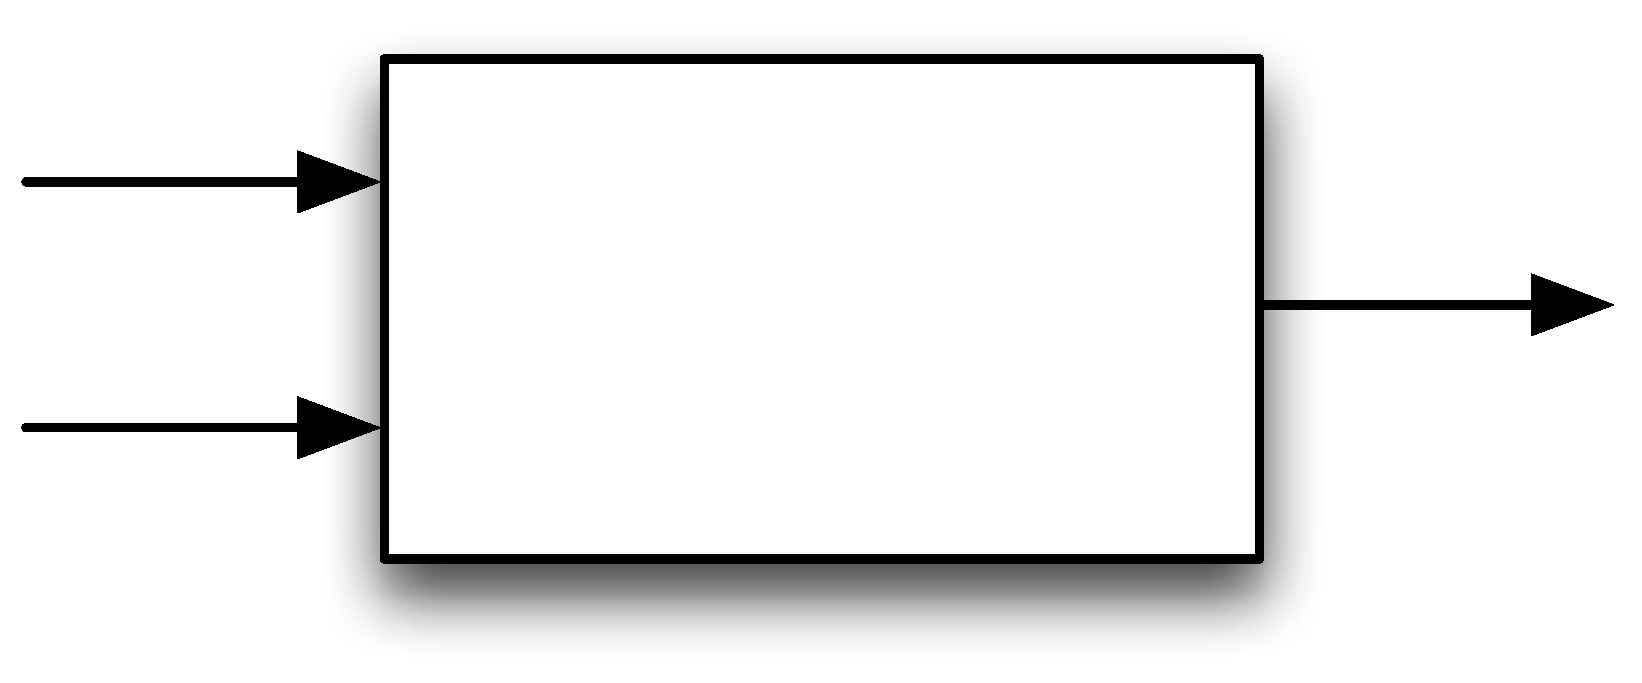
\includegraphics[width=2.5in]{Pictures/functionPic.pdf}
\end{center} 
The function gives an \textbf{output}\index{output} value which depends upon 
the \textbf{input}\index{input} value(s).
We will often also use the term {\bf result}\index{result}
for the output, and the terms {\bf arguments} or\index{argument}
{\bf parameters}\index{parameter} for the inputs. 

A simple example of a function is addition, \texttt{+}, over numbers.
Given input values \texttt{12} and \texttt{34} the corresponding output will be 
\texttt{46}.
\begin{center}
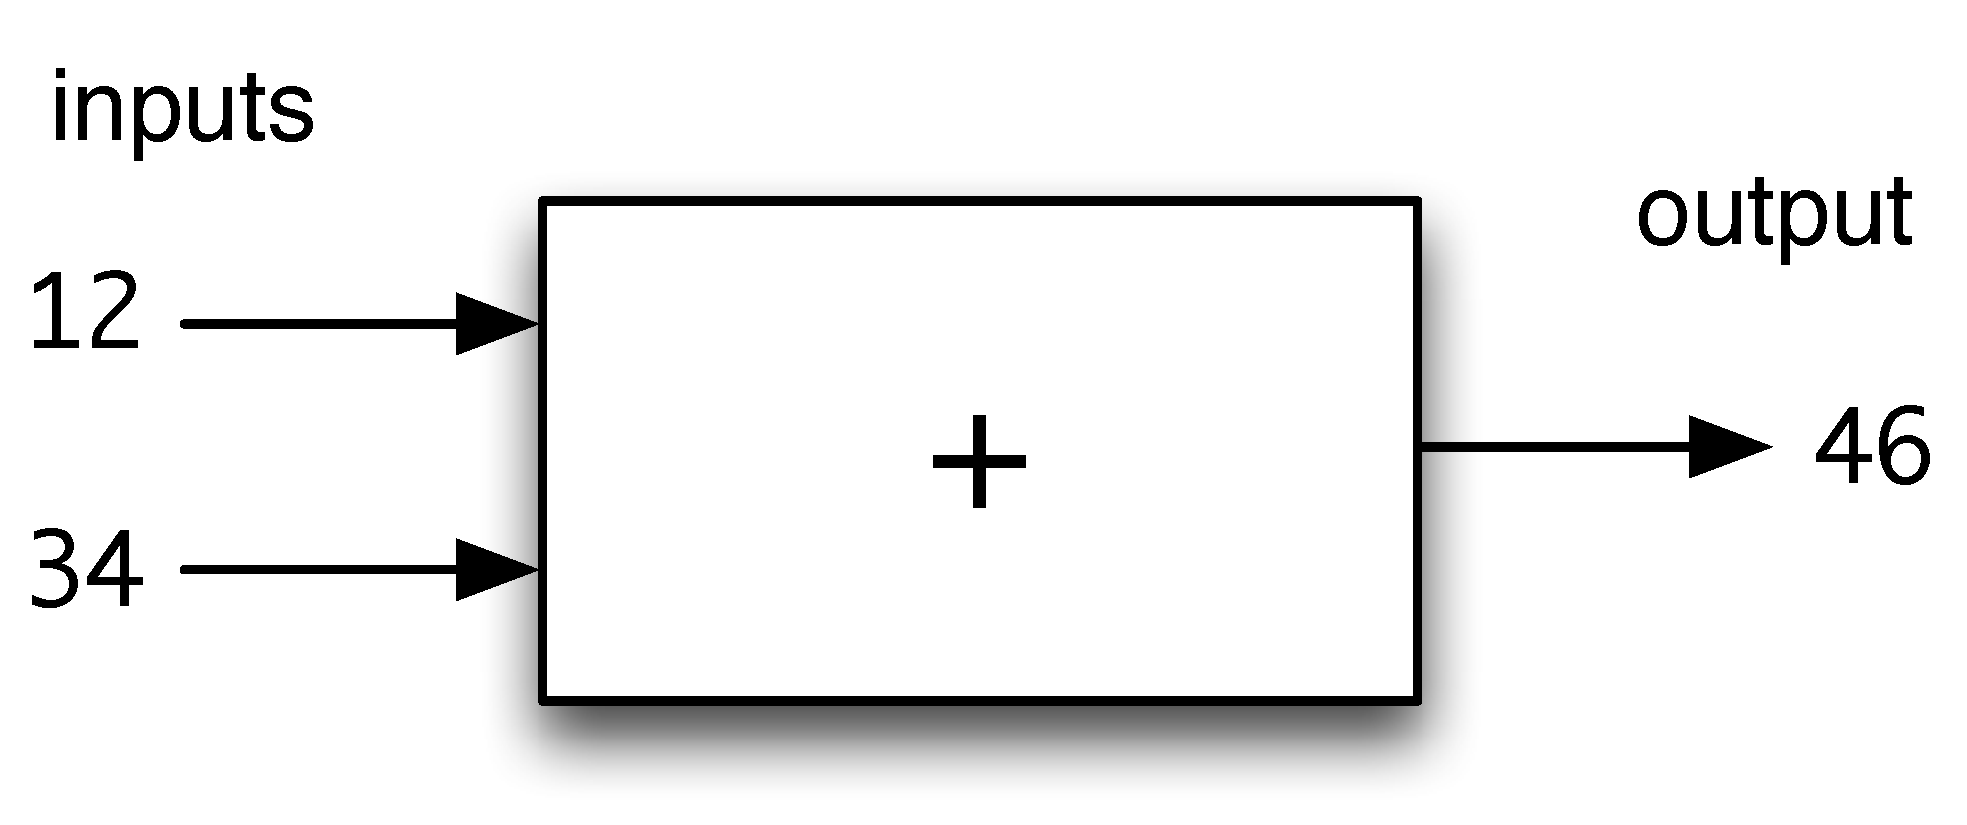
\includegraphics[width=3.0in]{Pictures/addFunPic.pdf}
\index{addition!function diagram}
\end{center} 
The process of giving particular inputs to a function is called \textbf{function
application}\index{application|see{function application}}\index{function application}, and
\texttt{(12 + 34)} represents the application of the function \texttt{+}\minx{+} to
\texttt{12} and \texttt{34}.

Addition is a mathematical example, but there are also functions in
many other situations; examples of these include
\label{examples1}  
\begin{titemize}
\item a function giving the distance by road ({\em output}) between two cities
({\em inputs});
\item a supermarket check-out program, which calculates the bill
({\em output}) from a list of bar codes scanned in ({\em input}); and
\item a process controller, which
controls valves in a chemical plant. Its inputs are the information from
sensors, and its output the signals sent to the valve actuators.
\end{titemize}
Different paradigms are characterized by the different tools
which they provide for modelling. In a functional programming language we'll focus on values -- such as bar codes and bills -- and the functions which work over them -- giving the total of a bill, say. We'll also see this
in our running example of pictures, which we look at next.

\section{Pictures and functions}
\label{picturesFuns}
\index{case studies!pictures|see{pictures}}
\index{pictures|(}


Let's take our first look at how pictures might be modelled.
First of all, we want to show that many common
relationships between pictures are modelled by functions; in the remainder of 
this section we consider a series of examples of this.

Reflection in a vertical mirror will relate two pictures, and we
can model this by a function \texttt{flipV}:\minx{flipV}
\begin{center}
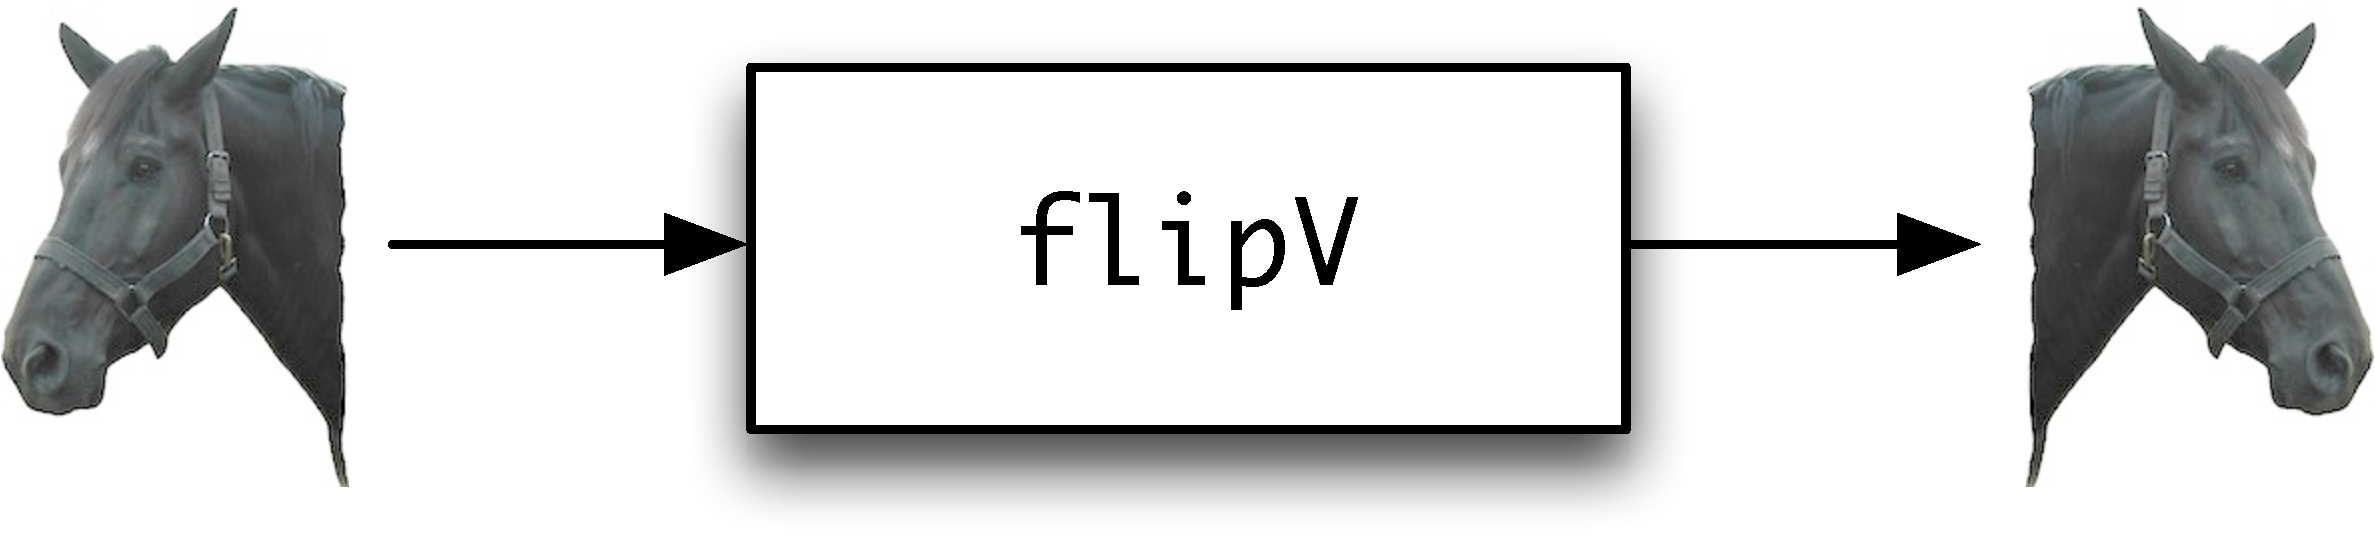
\includegraphics[width=3.5in]{Pictures/flipV.pdf}
\end{center}
where we have illustrated the effect of this reflection on the `horse'
image.
In a similar way we have a function \texttt{flipH} to represent flipping in a
horizontal mirror. 
Another function models the
inversion of the colours in a (monochrome) image:
\begin{center}\minx{invertColour}
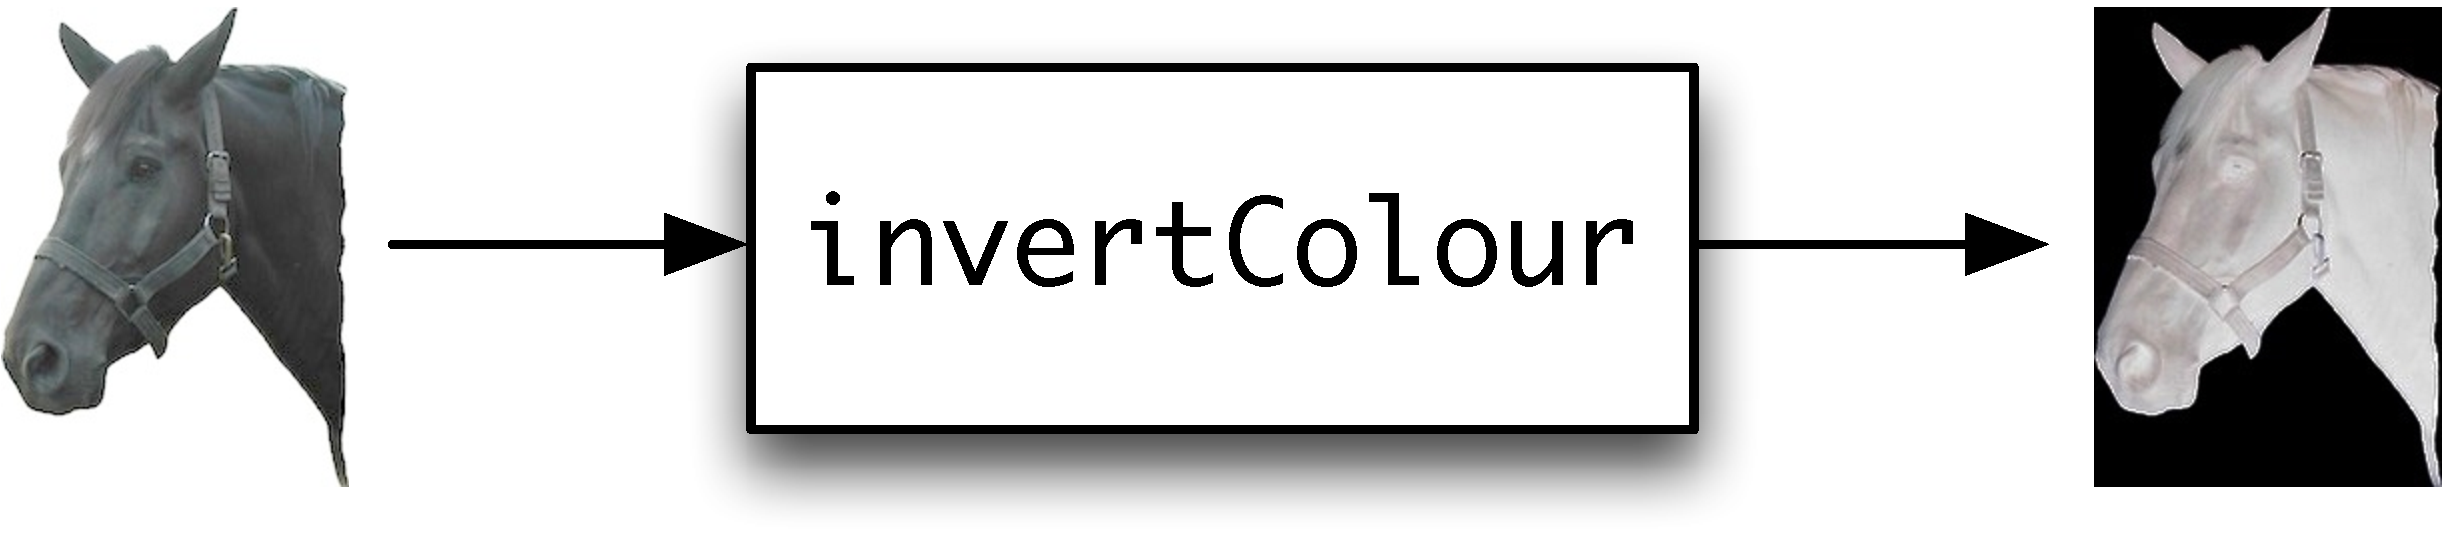
\includegraphics[width=3.8in]{Pictures/reverseVideo.pdf}
\end{center}
Some functions will take two arguments, among them a function to scale
images,
\begin{center}\index{scale@\texttt{scale}}
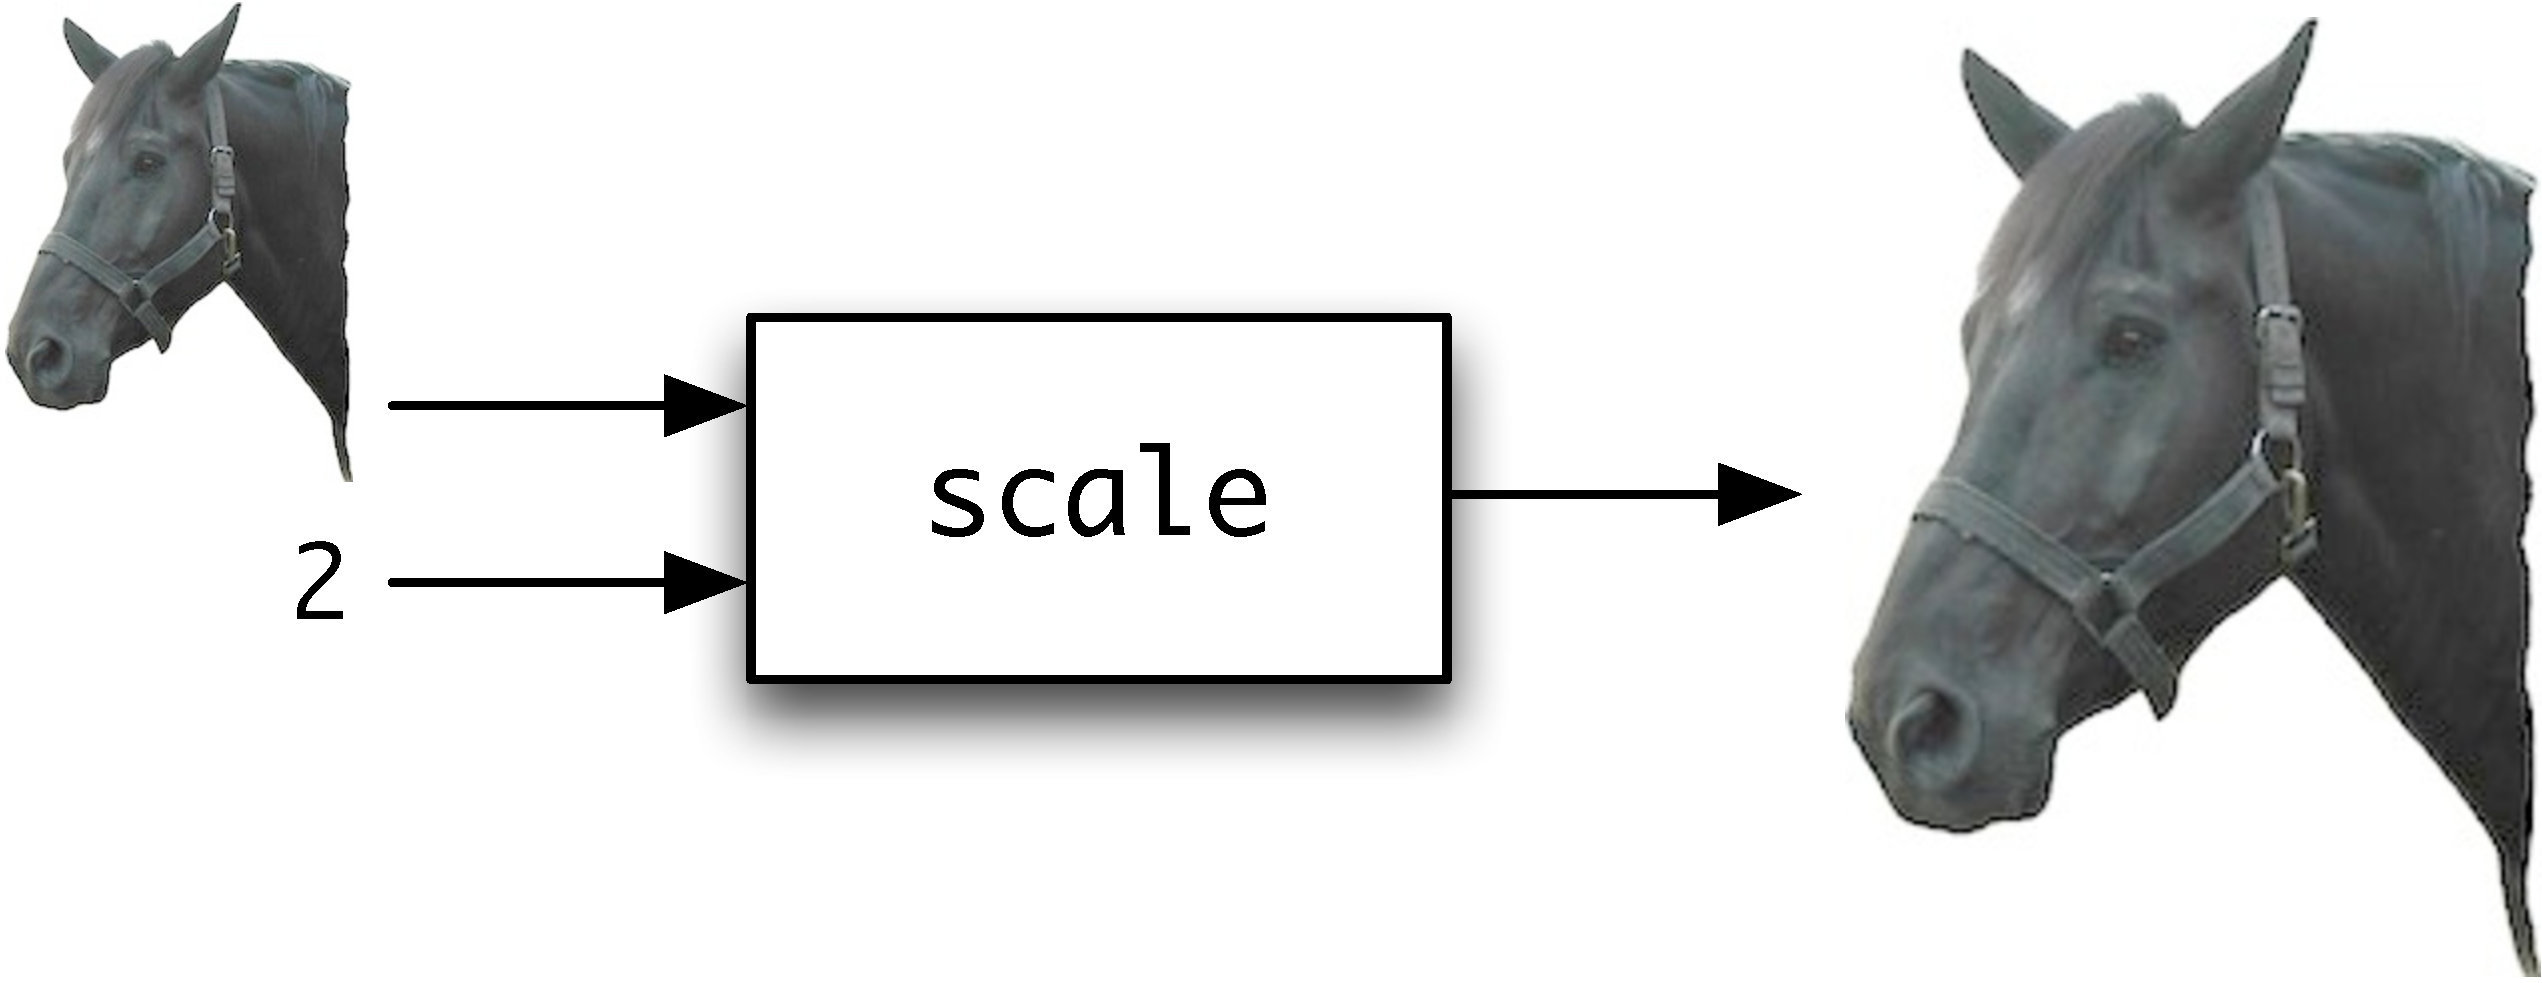
\includegraphics[width=3.8in]{Pictures/scale2.pdf}
\end{center}
a function to put one picture above another,
\begin{center}\minx{above}
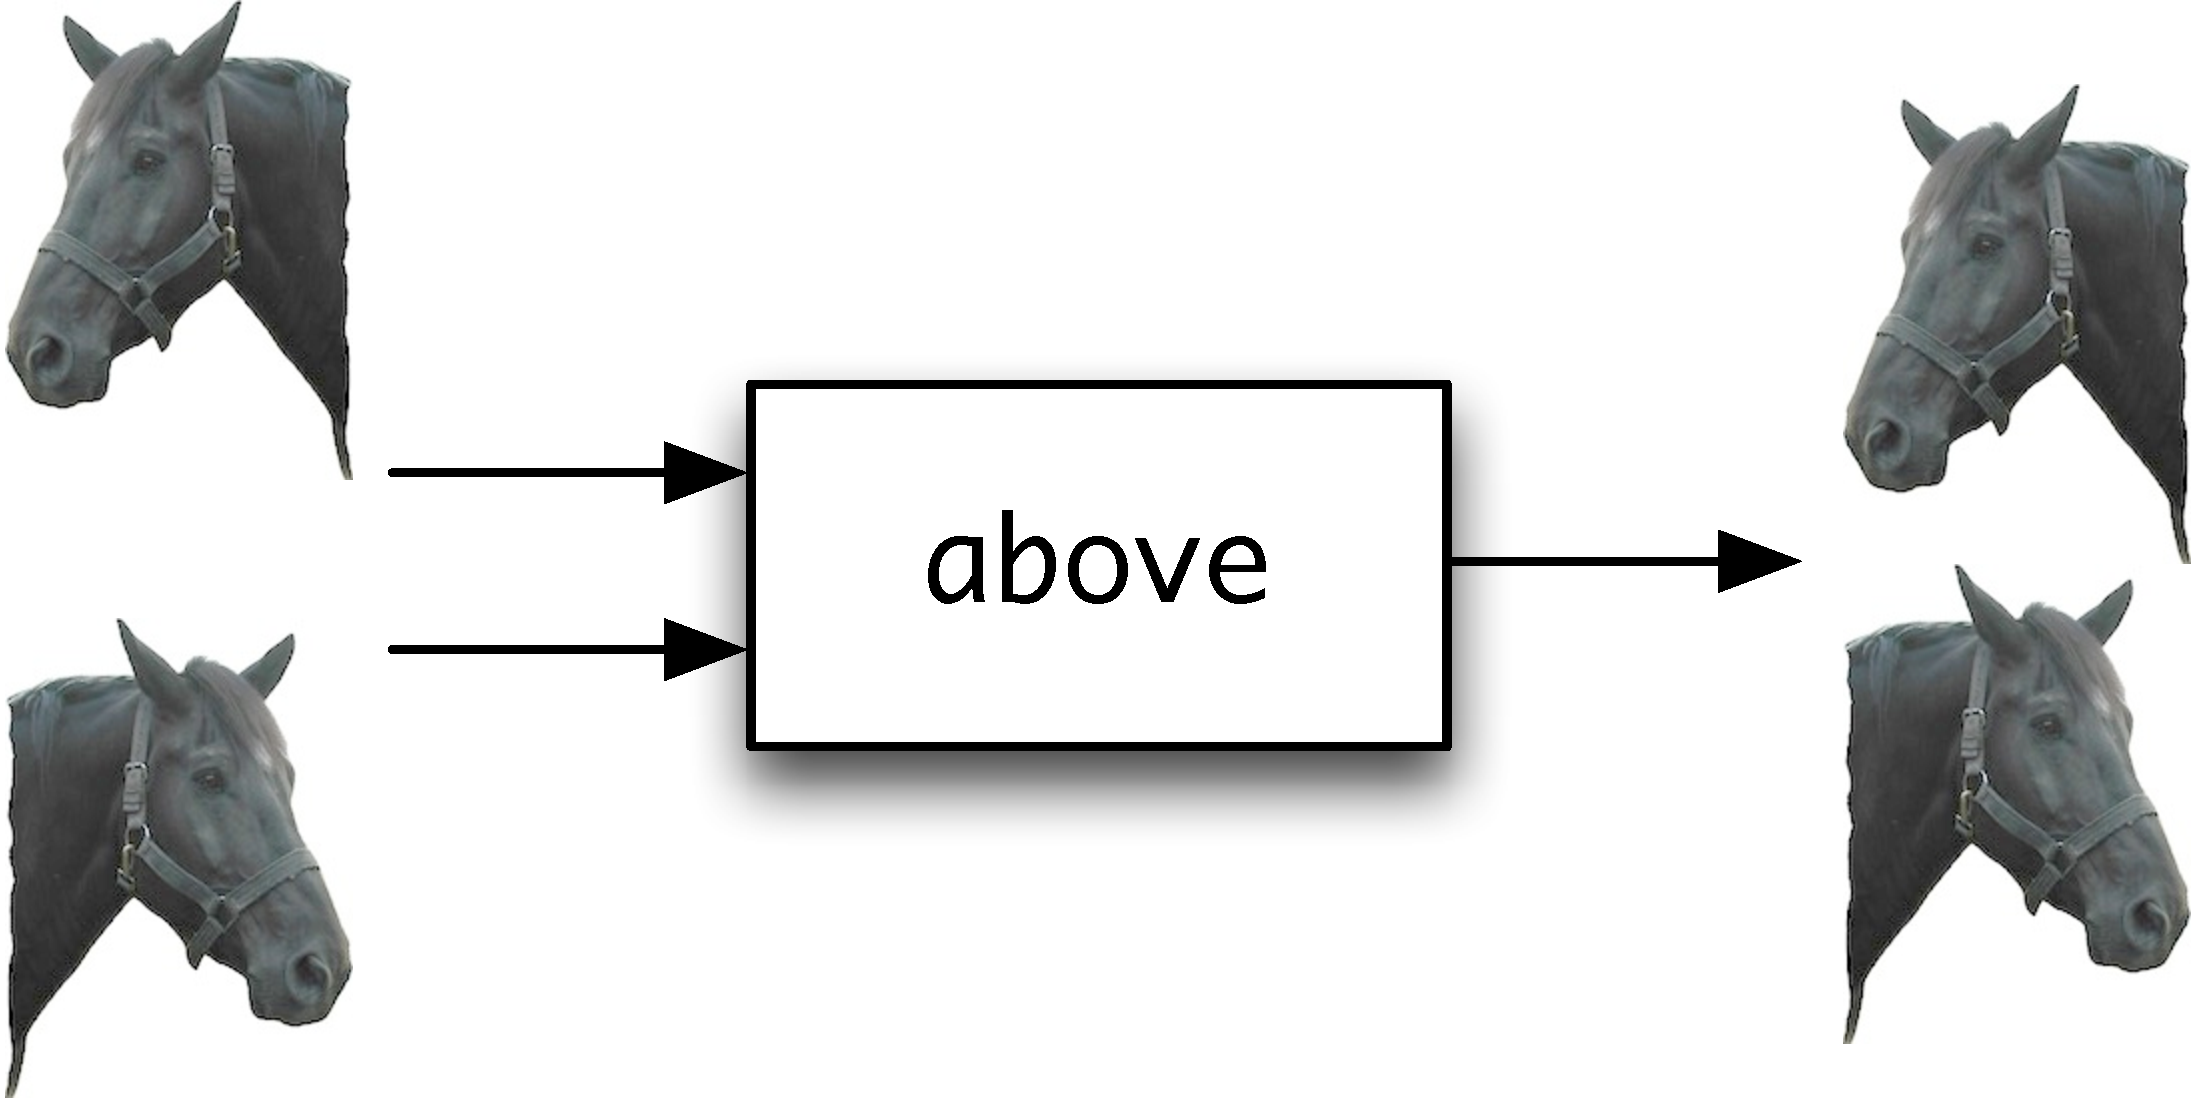
\includegraphics[width=3.4in]{Pictures/above.pdf}
\end{center}
and a function to place two pictures side by side.
\begin{center}\minx{beside}
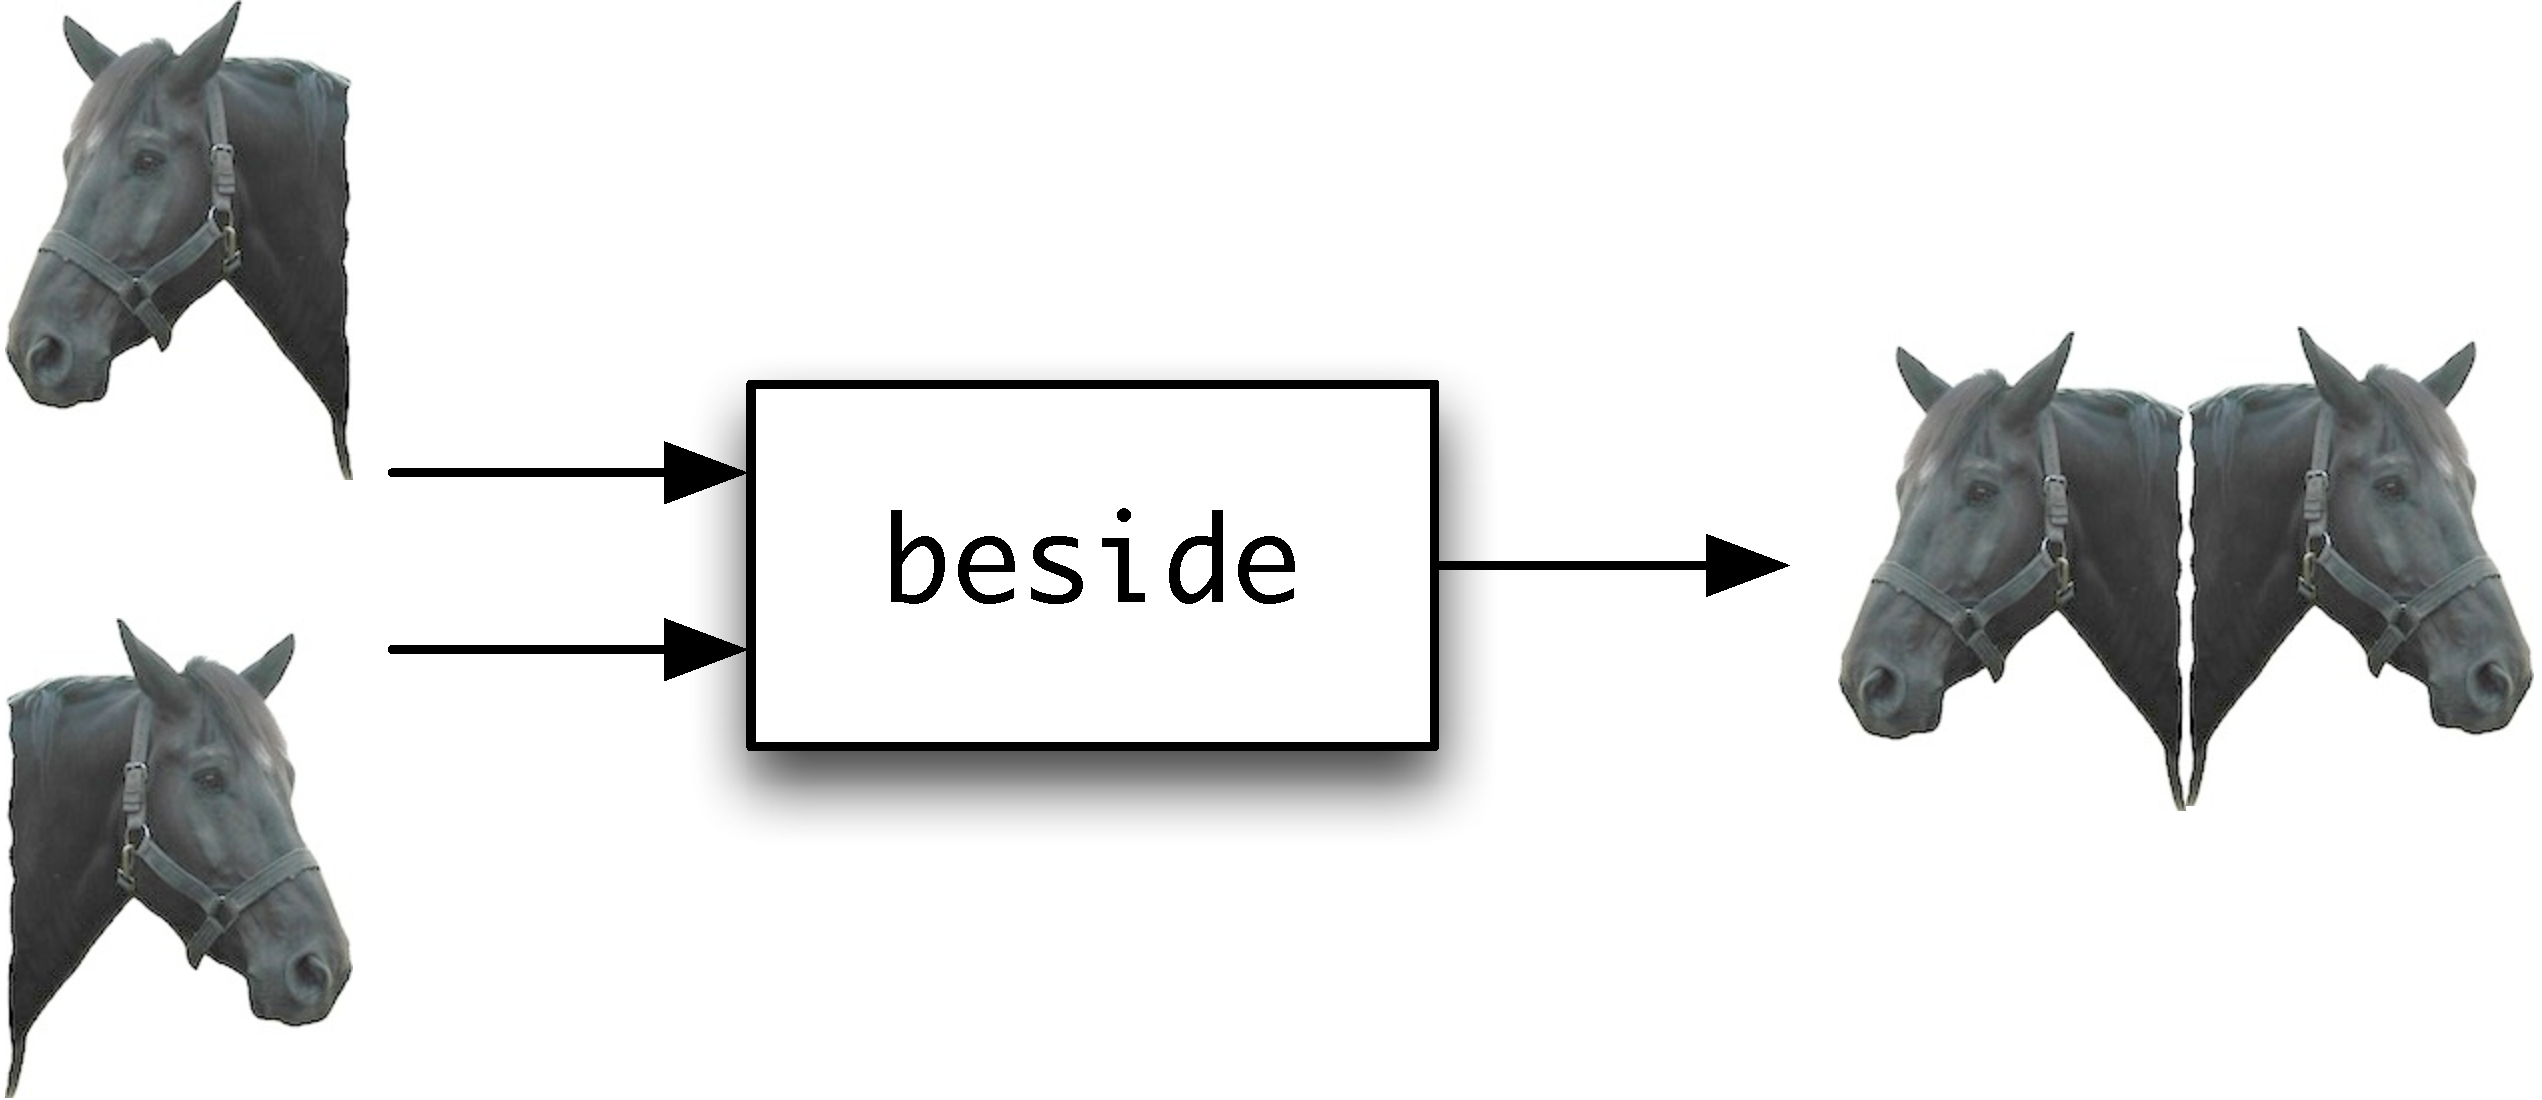
\includegraphics[width=3.8in]{Pictures/sideBySide.pdf}
\end{center}
All the functions here show that functions take a number of inputs (or arguments, parameters) and produce an output (or result) that depends on those inputs. What's more, this result only depends on those inputs, and will always give the same result for the same inputs. 

Before we can fully explain functional programming in Haskell, we
have to explain types, which we do now.

\section{Types}
\index{type}\label{typesIntro}

The functions which we use in functional programs will involve all sorts of
different kinds of value: the addition function \texttt{+} will combine two
numbers to give another number; \texttt{flipV}\minx{flipV} will transform a picture
into a picture; \texttt{scale}\index{scale@\texttt{scale}} will take a picture and a number and
return a picture, and so on. 

A \textbf{type}\index{type} is a collection of values, such as numbers
or pictures, grouped together because although they are different --
\texttt{2} is not the same as \texttt{567} -- they are the same {\em sort\/} of thing, in
that we can do the same things to them. In particular, we can apply the same functions to them.  For instance, we can find the larger
of any two numbers, but it doesn't make sense to do this for two pictures or a number and a picture. 
 
Each of the functions we have looked at so far will accept inputs from particular types, and give a result of a particular type too. If we look at the addition function, \texttt{+}, it only makes sense to add two scnumbers
but not two pictures, say. 
This is an example of the fact that the functions we have been talking about
themselves have a type, and indeed we can illustrate this diagrammatically:
\begin{center}\minx{+}\minx{Int}
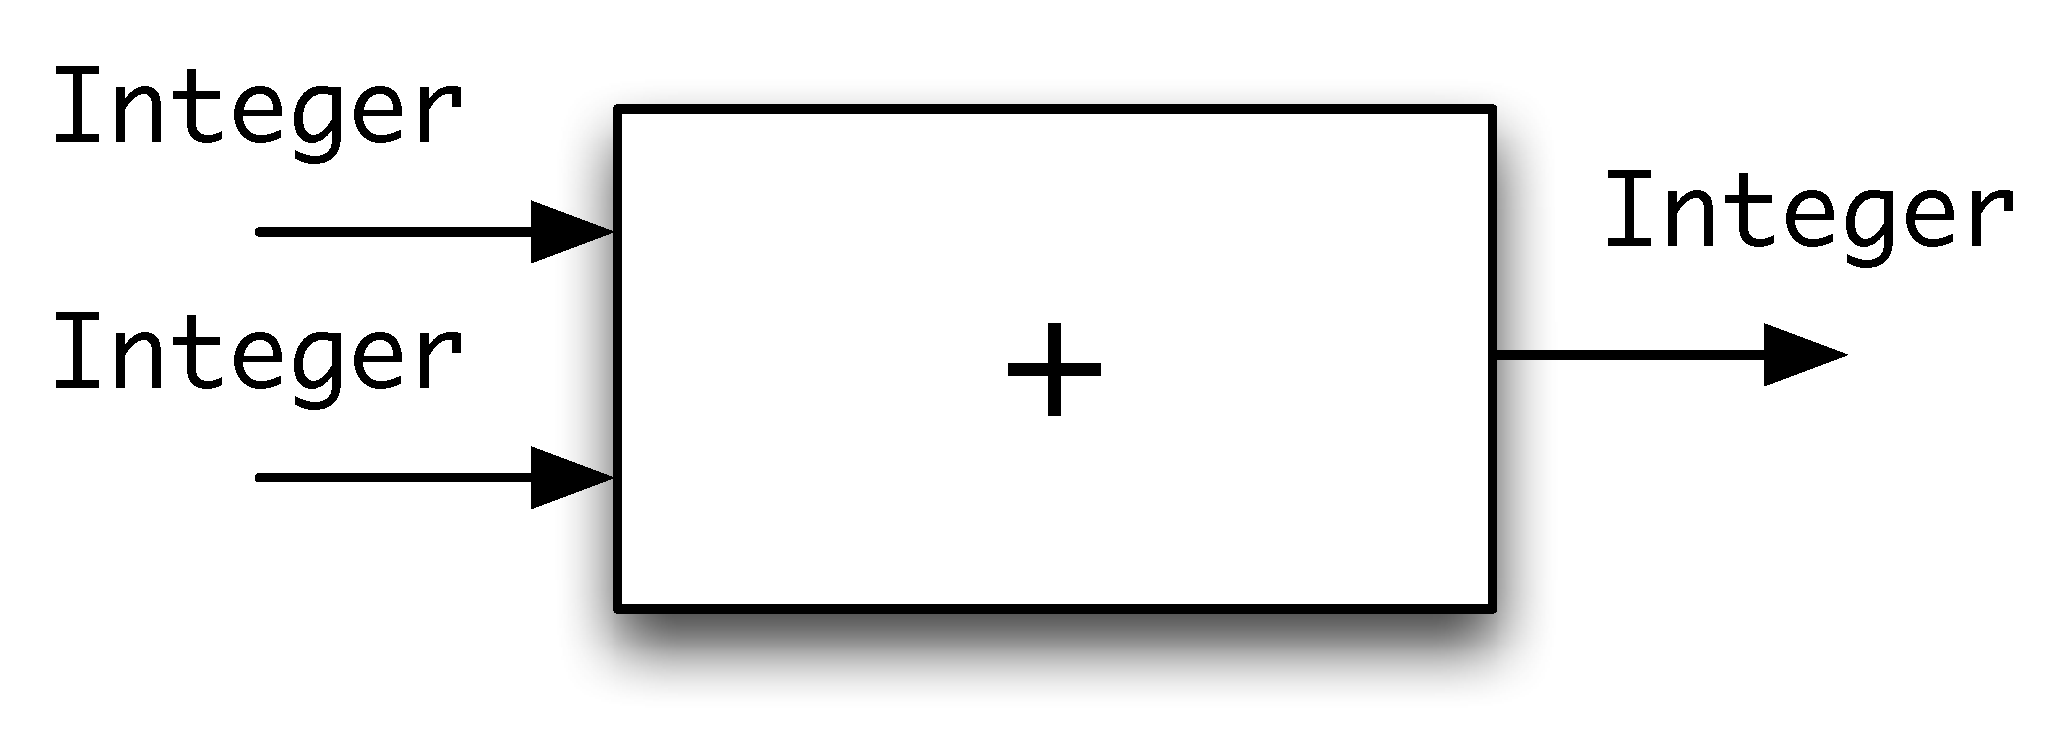
\includegraphics[width=3.0in]{Pictures/addFunPic2.pdf}\end{center}
\index{addition!type diagram}
The diagram indicates that \texttt{+} takes two whole numbers (or
\texttt{Integers})\minx{Integer} as arguments and gives an \texttt{Integer} as a result. In
a similar way, we can label the \texttt{scale} function
\begin{center}\index{scale@\texttt{scale}}
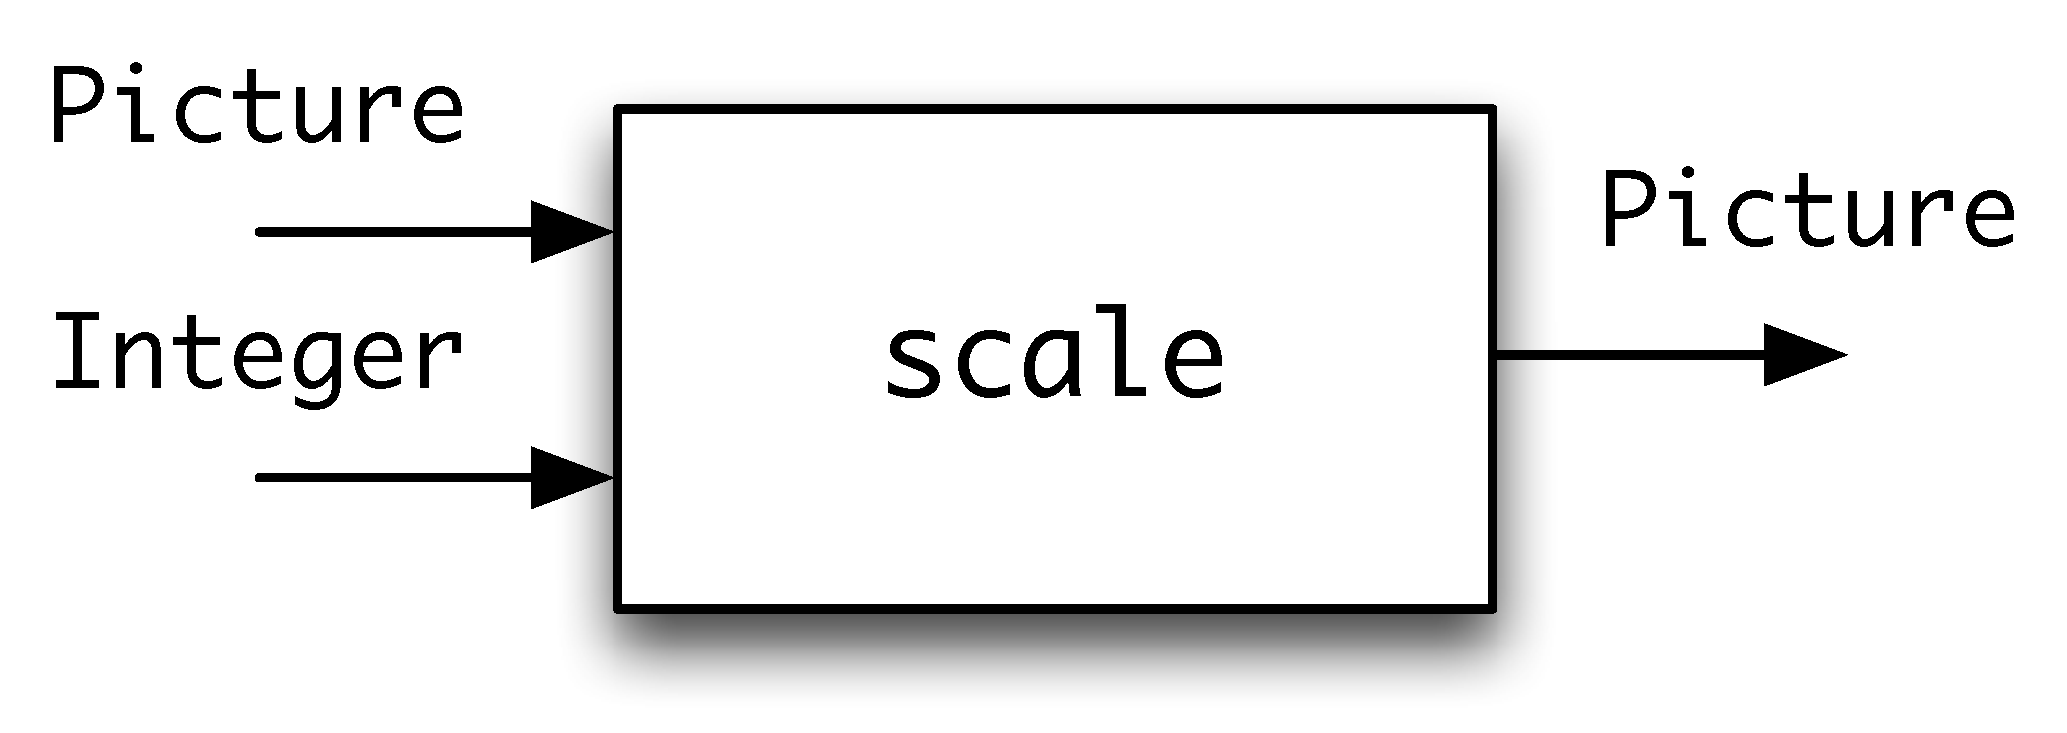
\includegraphics[width=3.0in]{Pictures/scaleType.pdf}
\end{center}\index{scale@\texttt{scale}!type diagram}
to indicate that its first argument is a \texttt{Picture}\minx{Picture} and its second
is an \texttt{Integer}, with its result being a \texttt{Picture}. We can see an example of this here, where \texttt{above} is correctly applied to two \texttt{Pictures}
\begin{center}\minx{above}
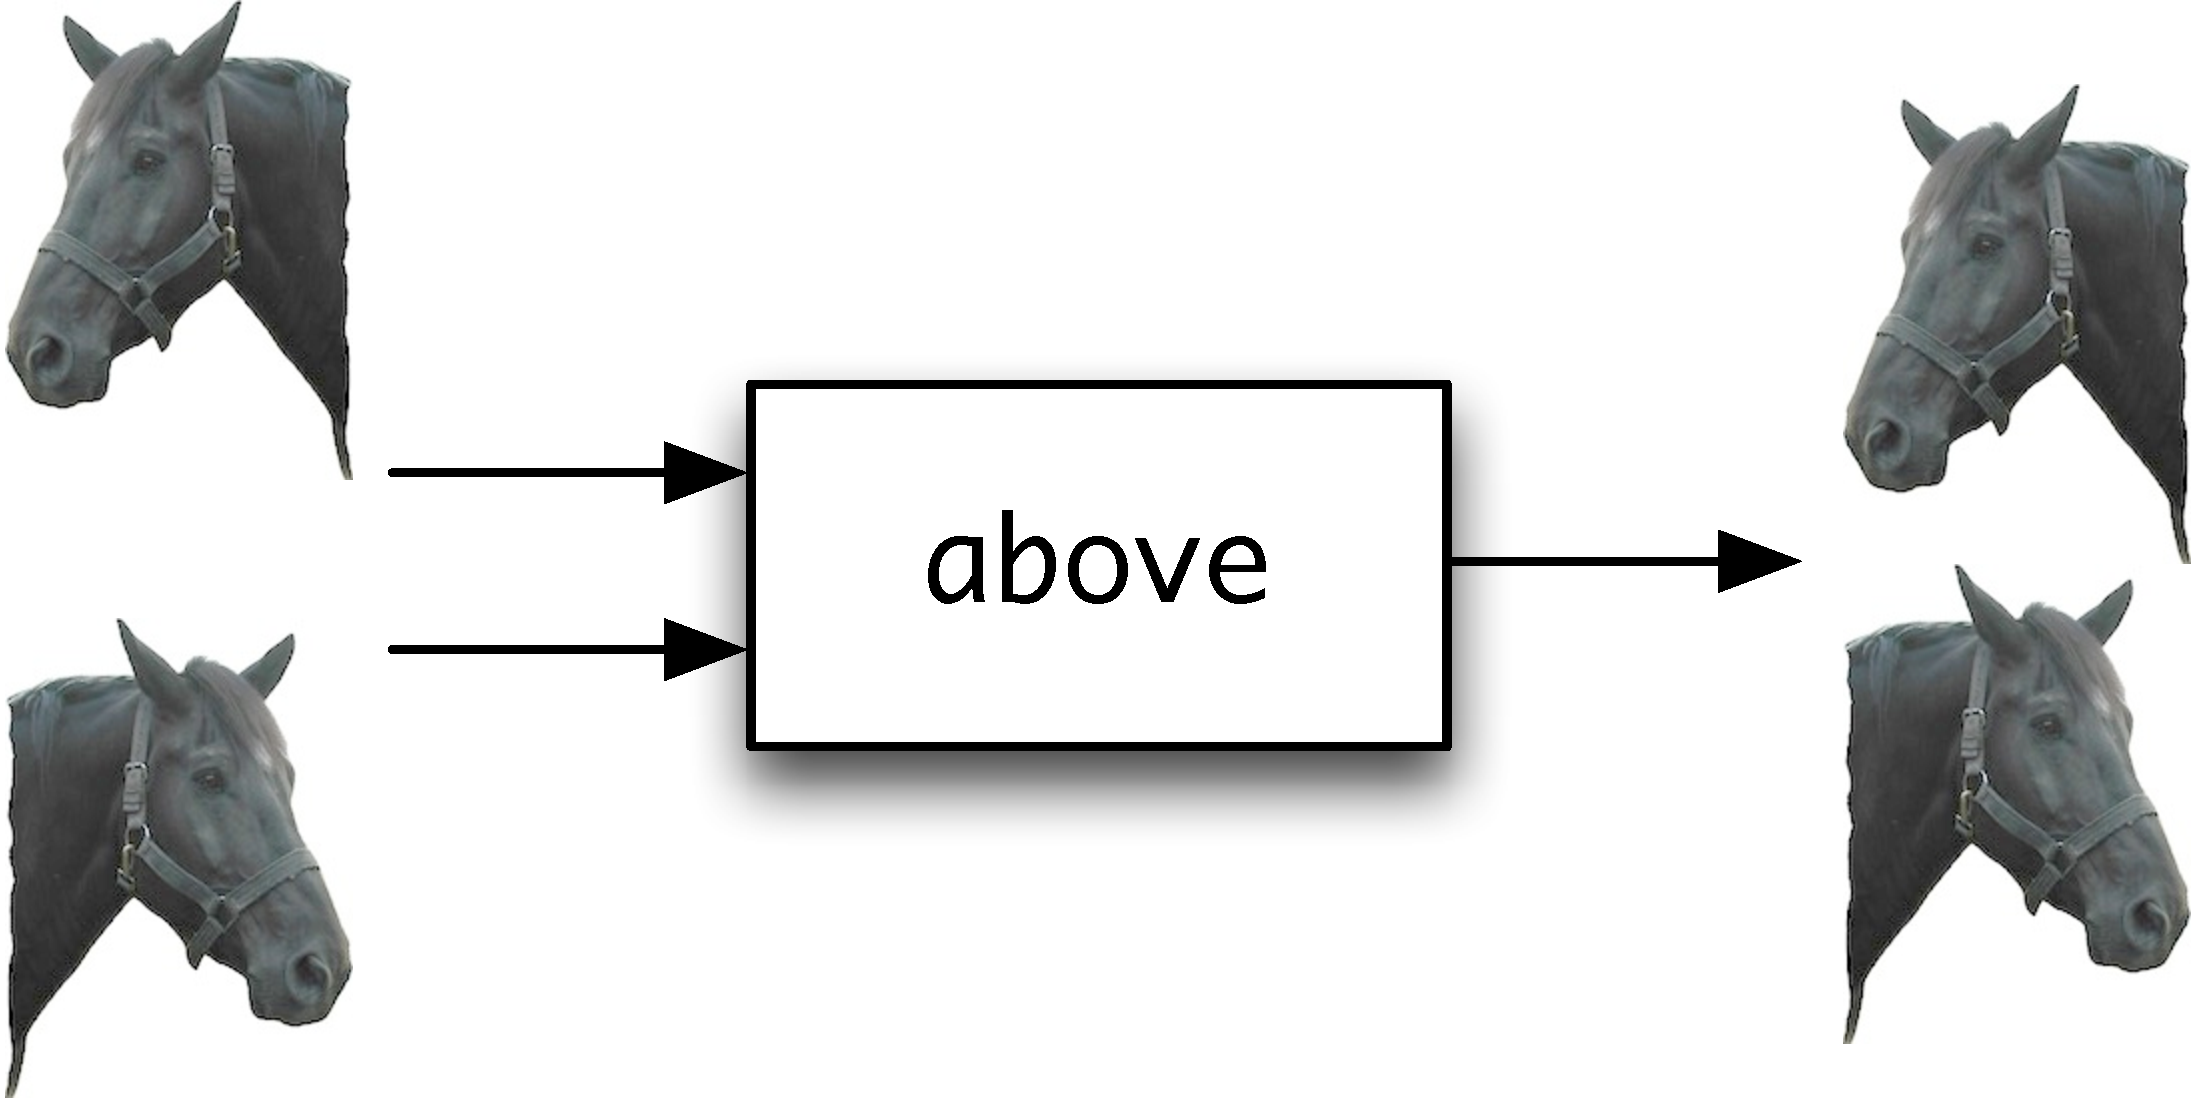
\includegraphics[width=3.4in]{Pictures/above.pdf}
\end{center}
but when applied to a \texttt{Picture} and an \texttt{Integer} a \textbf{type error} occurs, indicating that we have made a mistake:
\begin{center}\minx{above}
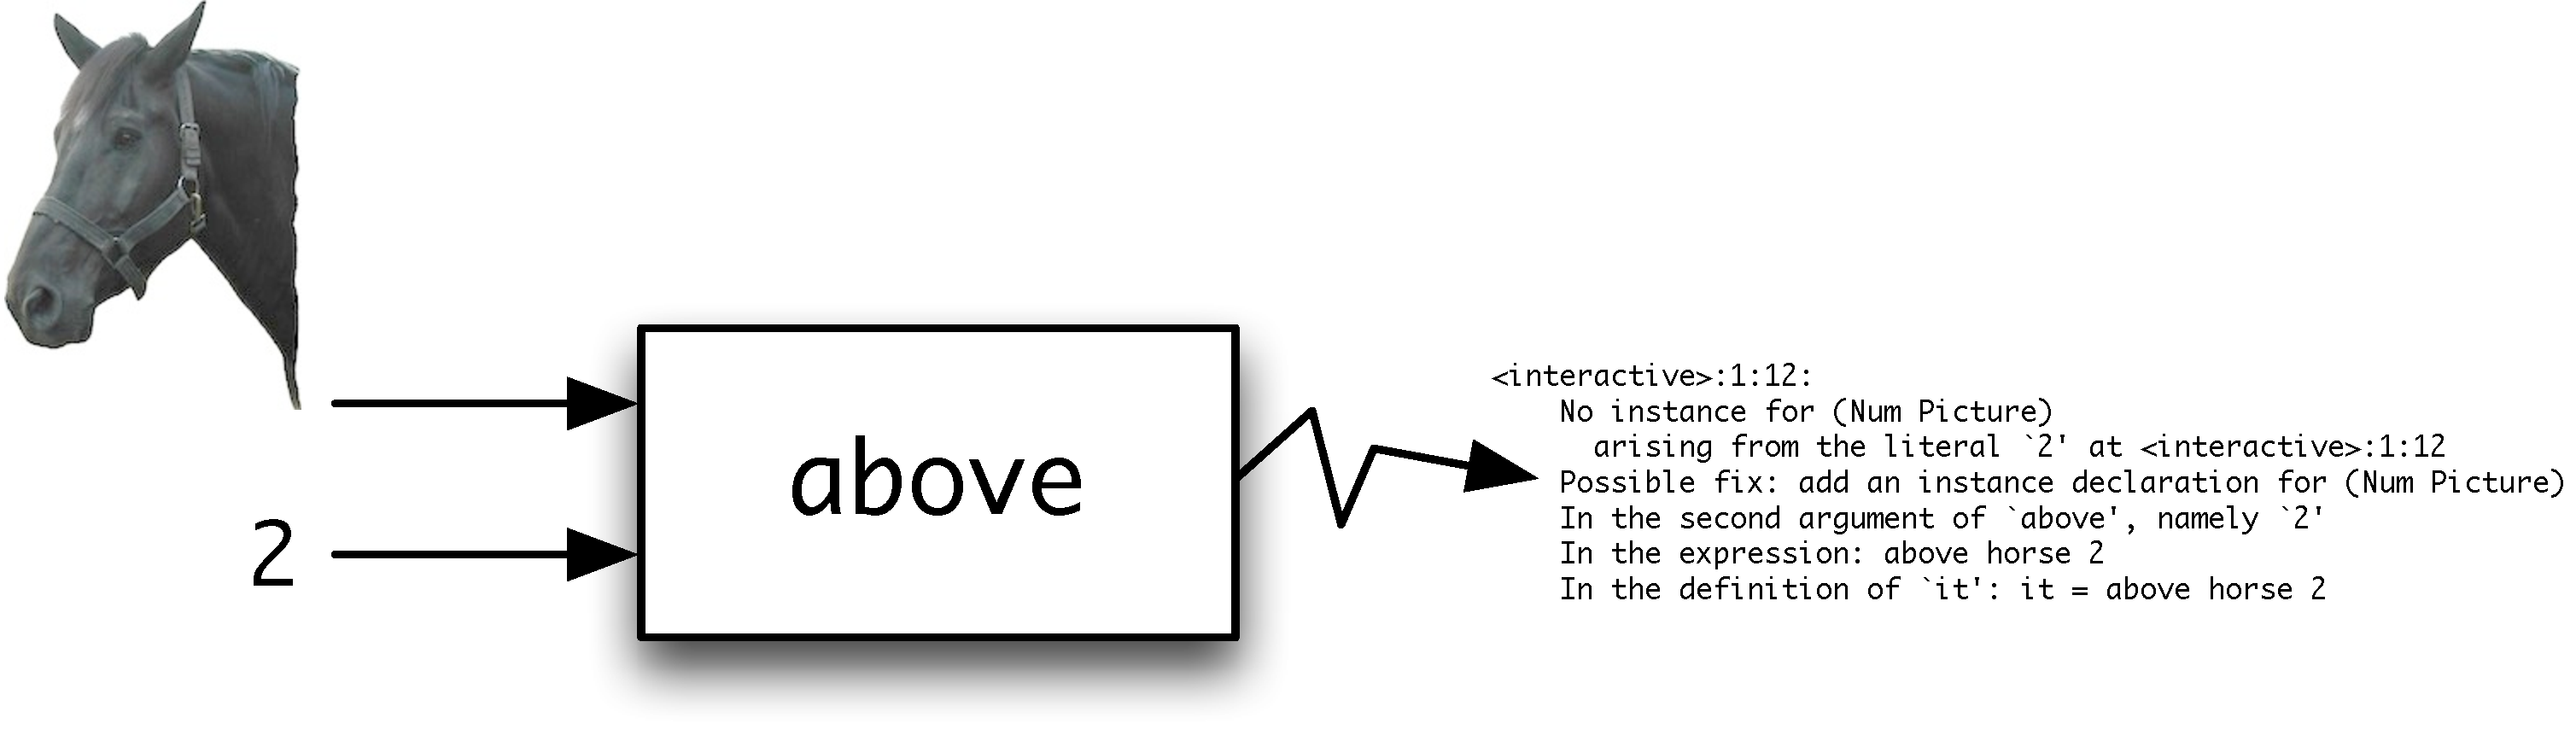
\includegraphics[width=5.0in]{Pictures/aboveError.pdf}
\end{center}
We have now explained two of the central ideas in functional
programming: a type is a collection of values, like the whole numbers or
integers; a function
is an operation\index{operation} which takes one or more
arguments to produce a result. The two concepts are linked: functions will operate over 
particular types:
a function to scale a picture will take two arguments, one of type \texttt{Picture} and
the other of type \texttt{Int}, and return a \texttt{Picture}. 

In modelling a
problem situation -- often called a problem \textbf{domain}\index{domain} -- types represent the things\footnote{I have not used the word `object' here because that has a technical meaning in OO languages; you could use it, but just remember it's meant in the non-technical sense here.} in the domain, while functions will represent what can be done to transform or manipulate the objects. In the case of pictures, we'll have a type \texttt{Picture} to represent the pictures themselves, and functions give operations on pictures, such as placing one above another, or scaling a picture. 

A rough and ready rule is that types correspond to \emph{nouns}, while functions, which transform or combine values from these types, are like \emph{verbs}. We come back to types in Section
\ref{typesFP} below.
\index{pictures|)}


\section{The Haskell programming language}


Haskell\index{Haskell} \cite{haskell2010} is the particular functional programming language which
we use in this text. Haskell was first defined in 1990, and it has undergone a series of changes since then: the version as I write is Haskell 2010.

Haskell is named after Haskell B.\ Curry,\index{Curry, Haskell B.} who was one of the pioneers of
the $\lambda$ calculus (lambda calculus)\index{lambda calculus},
a mathematical theory of functions that has been an
inspiration to designers of a number of functional languages. 

The best place to find out about everything to do with Haskell -- including the language definition itself, implementations, libraries, resources, mailing lists, news and Haskell jobs -- is the \texttt{haskell.org} website:
\begin{center}
\index{Web site!for Haskell}\index{haskell.org}
\url{https://www.haskell.org/}
\end{center}
There are various implementations of Haskell; in this 
text we shall use \textbf{GHCi}\index{GHCi} \citeyear{GHCi}. `GHCi' is an abbreviation for `Glasgow Haskell Compiler interactive': work on the compiler was started when Simon Peyton Jones and Simon Marlow were at Glasgow University; they are now both at Microsoft  Research in Cambridge.
GHCi provides an excellent environment for the learner, since it is freely
available for PC, Linux and Mac OS X systems, it is efficient and compact
and has a flexible user interface.

GHCi is an interpreter\index{interpreter} -- which means loosely that 
it evaluates expressions step-by-step as we might on a piece of paper -- but it can also load code that has been compiled into machine language. So, GHCi combines the flexibility of an interpreter with the efficiency of a compiler,\index{compiler} 
allowing its programs to run with a speed similar to those
written in more conventional languages like C and C++. Details of other
different implementations of Haskell can be found in Appendix
\ref{OtherHS}, and a full description of all of them is available at the \texttt{haskell.org} page.


GHCi is installed, together with the \textbf{Cabal}\index{Cabal} \cite{Cabal} build tool, using \textbf{GHCup}\index{GHCup}, \url{https://www.haskell.org/ghcup/}, the toolchain installer that \texttt{haskell.org} itself recommends; we describe how to install it in Chapter \ref{getStart}. Libraries beyond those that come with GHC are available from an extensive online database, \textbf{HackageDB}\index{HackageDB} \cite{Hackage}, and Cabal makes it easy to download and install them: we describe how to work with the interactive version of GHC in the next chapter, and how to use Hackage and Cabal in Chapter \ref{progLists}.

All the programs and examples used in the text can be downloaded as the \texttt{Craft3e} package from Cabal and from the website for this book,
\begin{center}
\label{bookWeb}
\url{http://www.haskellcraft.com/}
\end{center}\minx{www.haskellcraft.com}\index{website}
This site also pulls together a collection of resources, further reading and other background materials for this text.

\section{Expressions and evaluation}
\label{exprEval}

In our first years at school we learn to \textbf{evaluate}\index{evaluation}
an \textbf{expression}\index{expression} like \texttt{(7 - 3) * 2}
\begin{center}
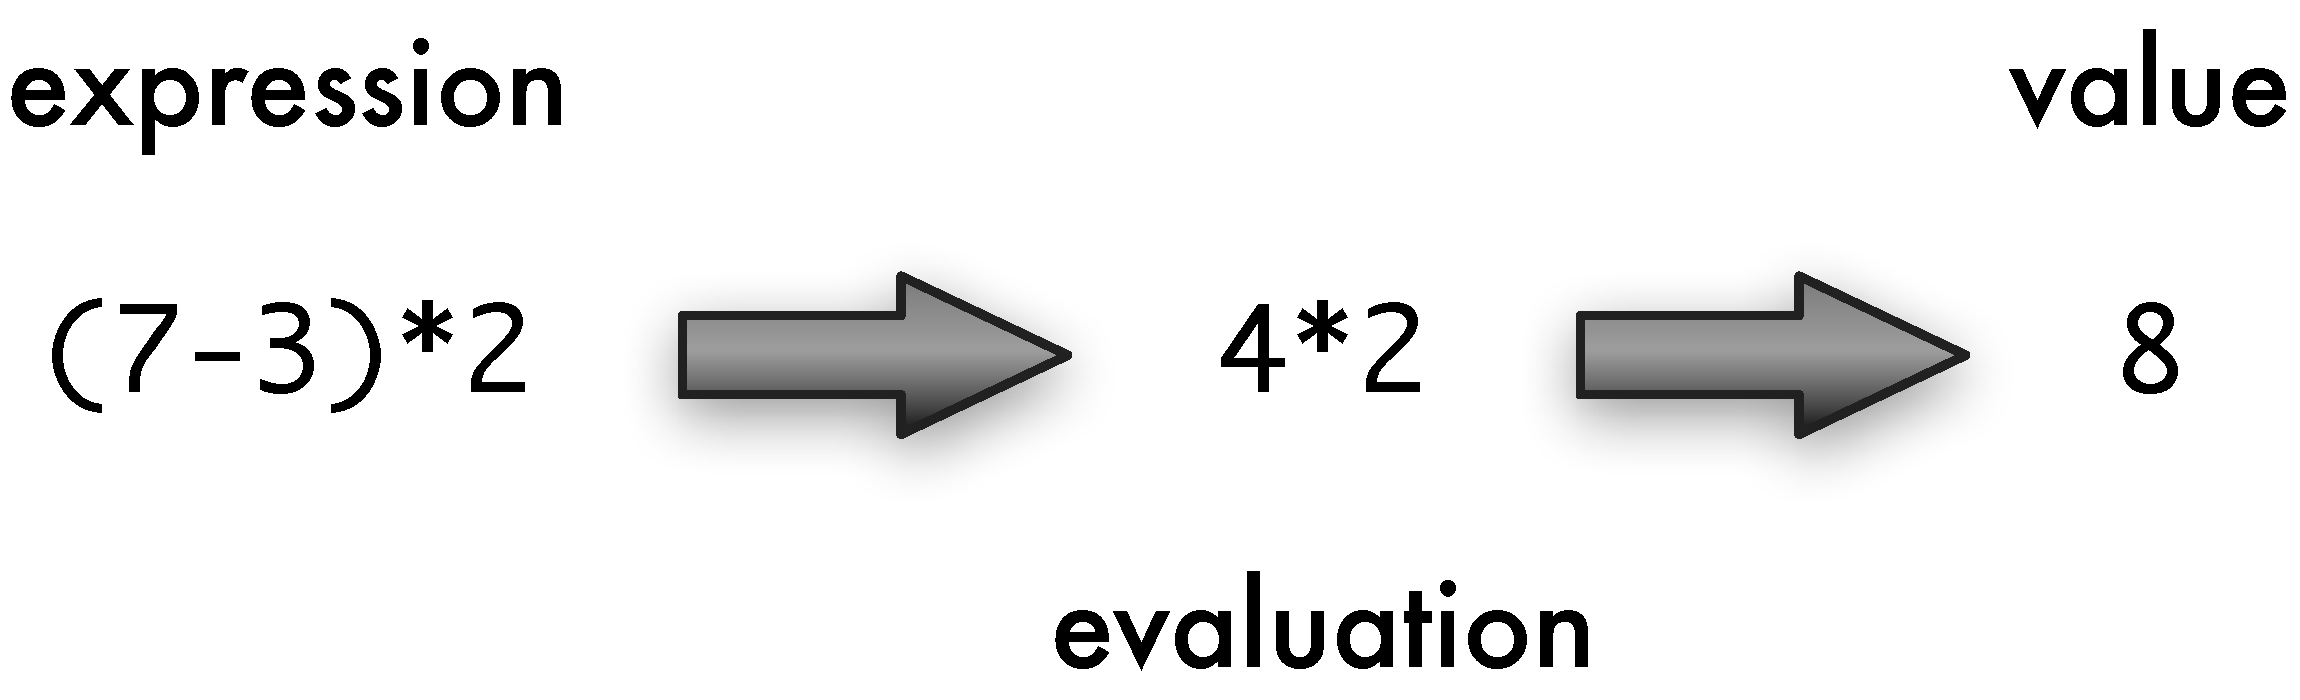
\includegraphics[width=3in]{Pictures/evaluation.pdf}
\end{center}
to give the \textbf{value}\index{value} \texttt{8}.
Expressions are built up by applying functions to numbers and other expressions built in the same way. In this particular example, the functions are subtraction \texttt{-}\minx{-} and multiplication \minx{*}\texttt{*}, and the numbers \texttt{7}, \texttt{3} and \texttt{2}; the value of the expression is a number.
This process of evaluation is automated in an electronic calculator.

In functional programming we do exactly the same: we evaluate expressions
to give values, but in those expressions we use functions which
model our particular problem. For example, in modelling pictures we will want
\index{pictures}
to evaluate expressions whose values are pictures.
If the picture\minx{horse}
\begin{center}
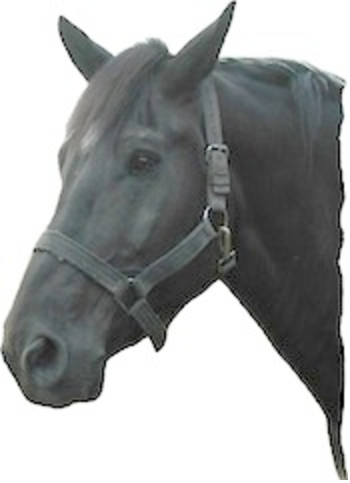
\includegraphics[width=0.6in]{Pictures/simplePic.pdf}
\end{center}
is called \texttt{horse}, then we can form an expression by applying the
function \texttt{flipV}\minx{flipV} to the horse. This function
application\index{function application} is written by putting the function
followed by its arguments, like this:
\begin{alltt}
flipV horse
\end{alltt}
and then evaluation will give
\begin{center}
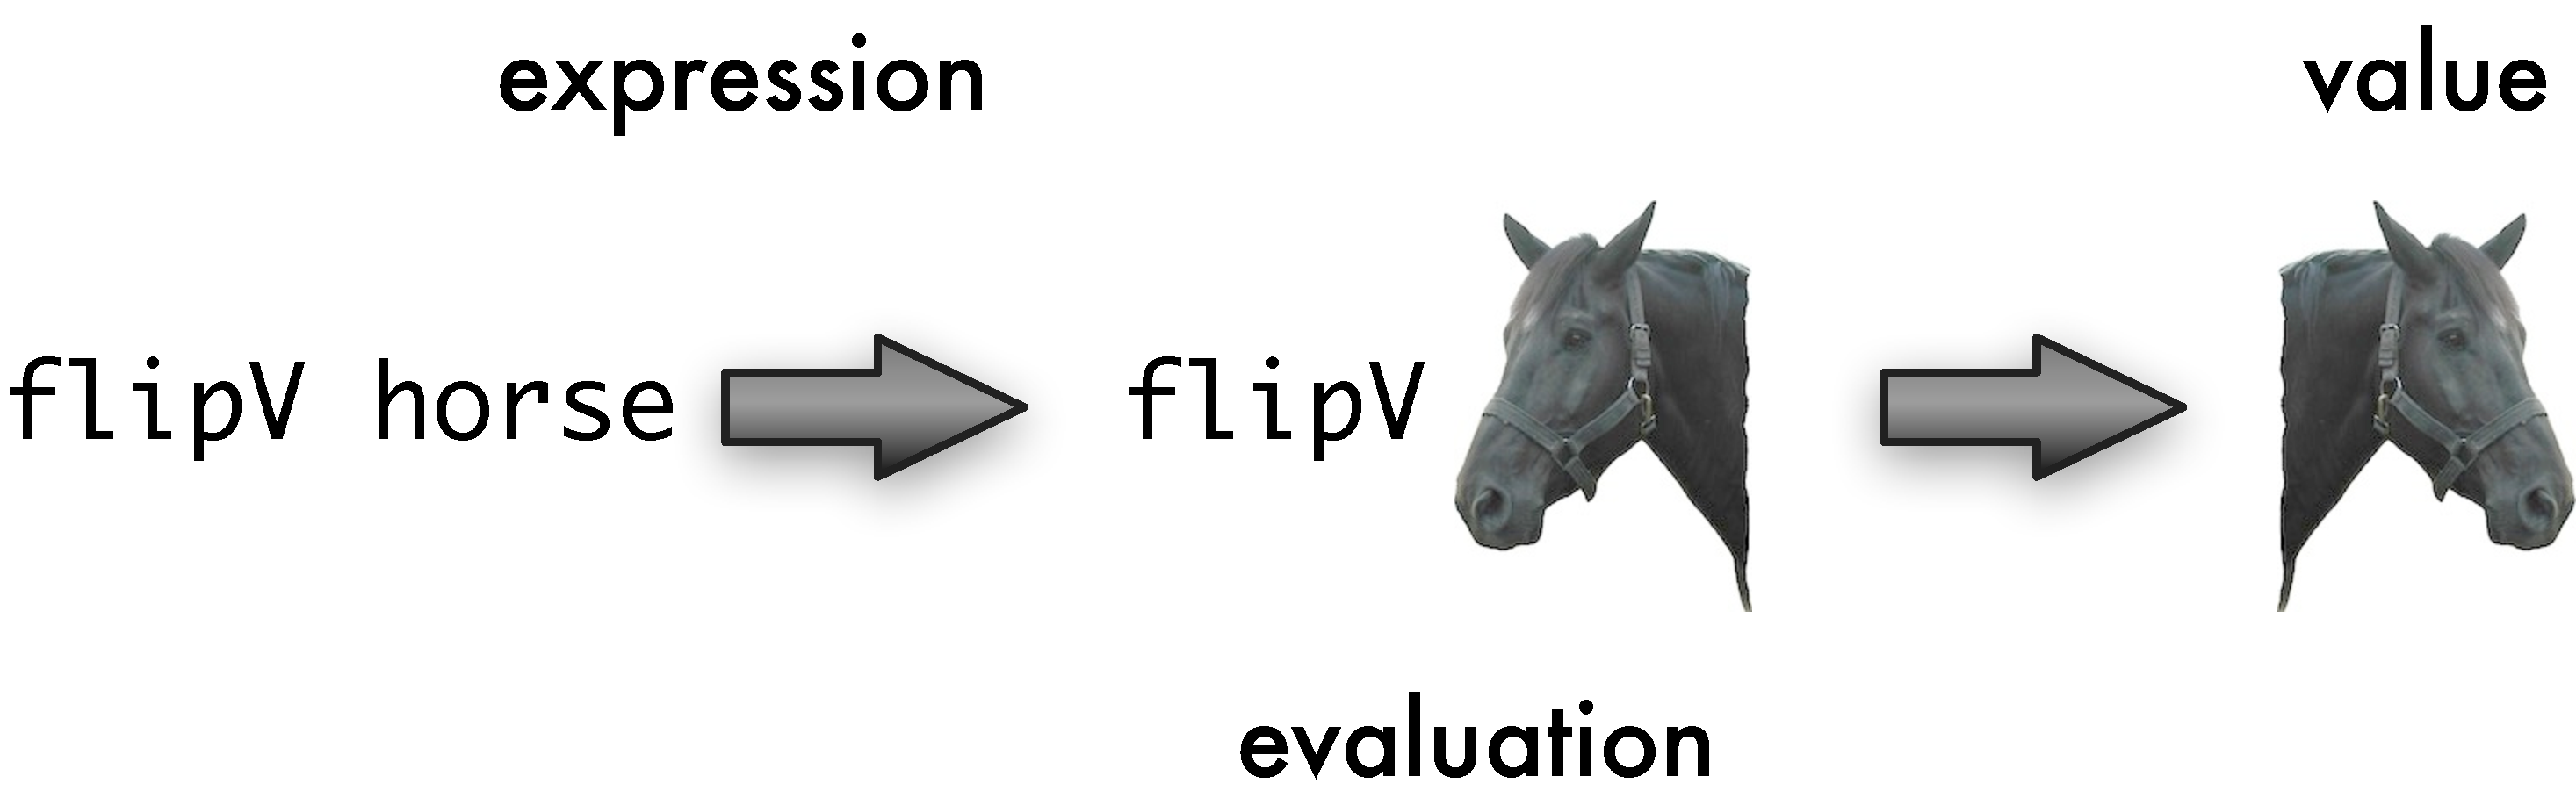
\includegraphics[width=3.8in]{Pictures/evaluation2.pdf}
\end{center}
A more complicated expression is
\begin{alltt}\minx{invertColour}
invertColour (flipV horse)
\end{alltt}
the effect of which is to give a horse reflected in a
vertical mirror -- \texttt{flipV horse} as shown above -- and then to invert
the colours in the picture to give
\begin{center}
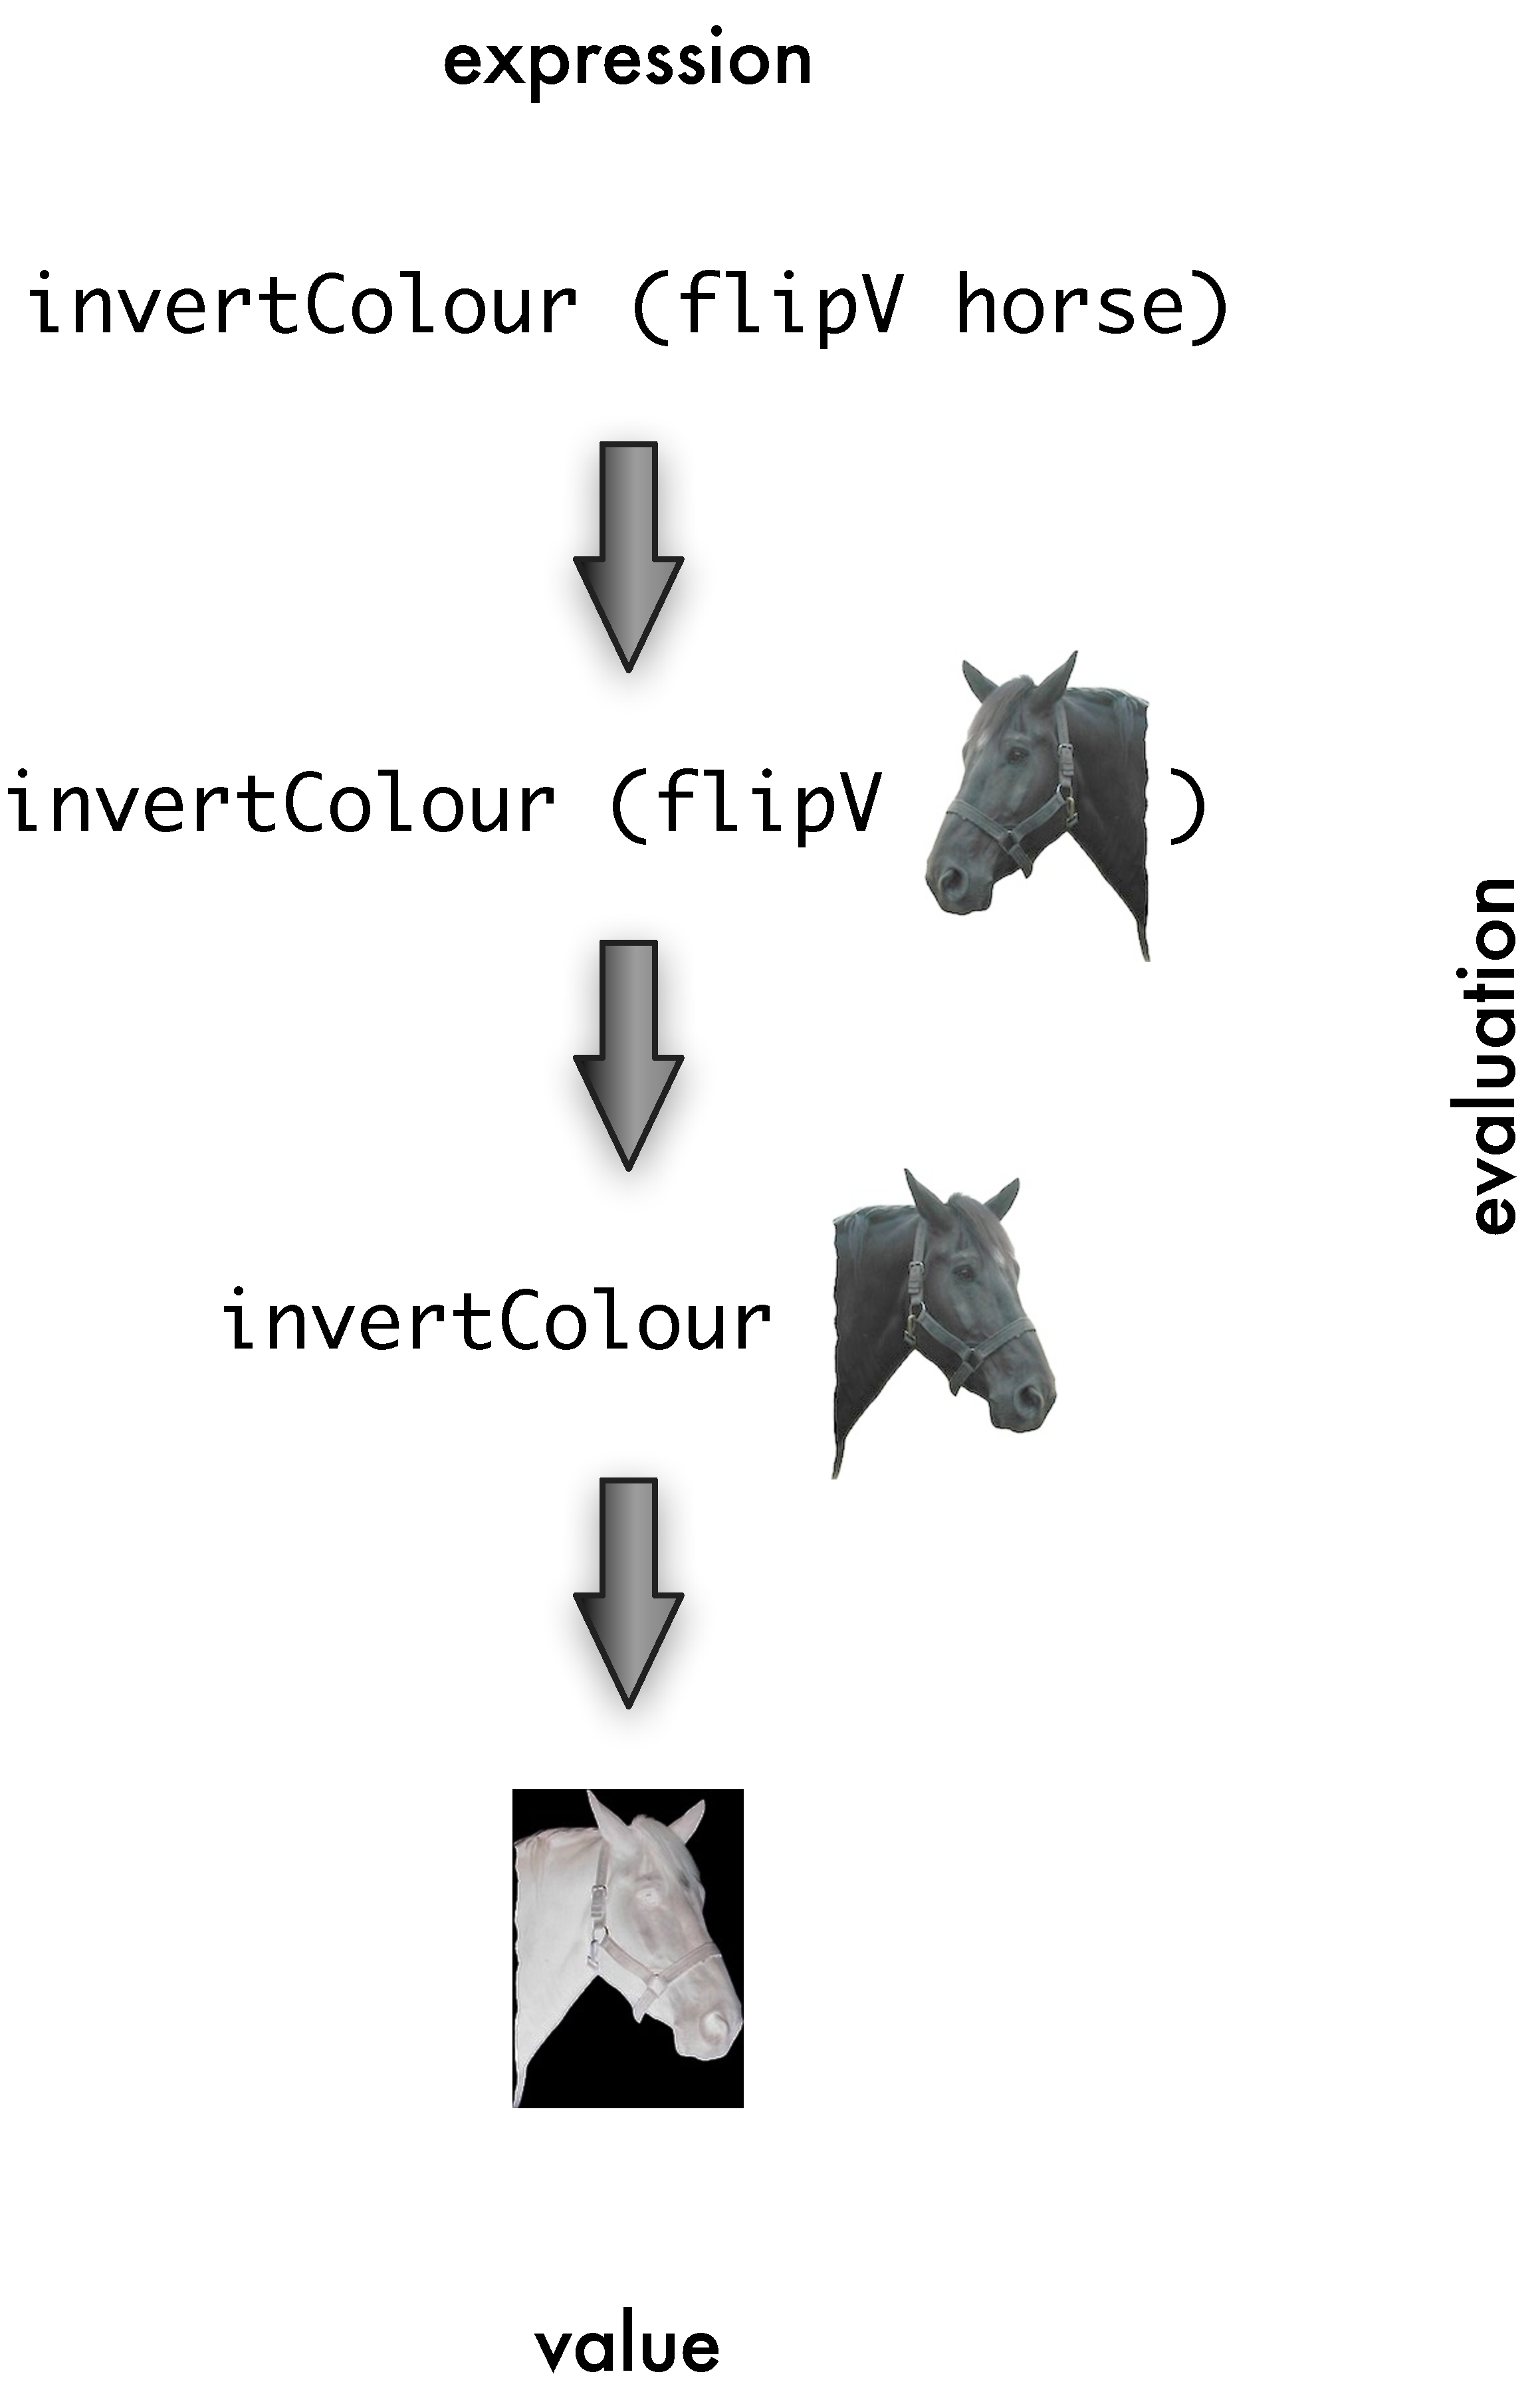
\includegraphics[width=2.8in]{Pictures/evaluation3.pdf}
\end{center}
To recap, in functional programming, we compute by evaluating
expressions which use functions in our area of interest. We can see an implementation of 
a functional language as something like an electronic calculator: we
supply an expression, and the system evaluates the expression to give
its value. The task of the programmer is to write the functions which
model the problem area.

So, a \textbf{functional
program}\index{functional program} is made up of a series of
\textbf{definitions}\index{definition} of functions and other values. 
We will look at how to write these definitions now.


\section{Definitions}
\label{defsIntro}

A functional program in Haskell consists of a number of
\textbf{definitions}\index{definition}. A Haskell
definition associates a \textbf{name}\index{name}
with a value of a particular \textbf{type}. 
We often use the word `\textbf{identifier}'\index{identifier} instead of `name': they mean exactly the same thing.

In the simplest
case a definition will look like this\minx{=}
\begin{alltt}
name :: type
name = expression
\end{alltt}
as in the example
\begin{alltt}
size :: Integer
size = 12+13
\end{alltt}
which associates the name on the left-hand side, \texttt{size}, with the value of the expression
on the right-hand side, \texttt{25}, a value whose type is \texttt{Integer}\minx{Integer}, the type of whole numbers
or integers. The symbol `\texttt{::}'\minx{::} can be read as ``is a / is an'', so the first line of the last definition reads `\texttt{size} is an \texttt{Integer}'.\index{reading `\texttt{::}'} Note also that names for functions and other
values begin with a \emph{small letter}, while type names begin with a \emph{capital
letter}.\index{name!value}\index{name!type}



Suppose that we are supplied with the definitions of \texttt{horse} and the various
functions over \texttt{Picture}\minx{Picture} mentioned earlier -- we will discuss in 
detail how to download these and use them in a program in Chapter \ref{getStart} -- we can
then
write definitions which use these operations over pictures. For example, we can say
\begin{alltt}\minx{blackHorse}
blackHorse :: Picture
blackHorse = invertColour horse
\end{alltt}
so that the \texttt{Picture} associated with \texttt{blackHorse} is obtained by
applying the function \texttt{invertColour} to the \texttt{horse},
thus giving
\begin{center}
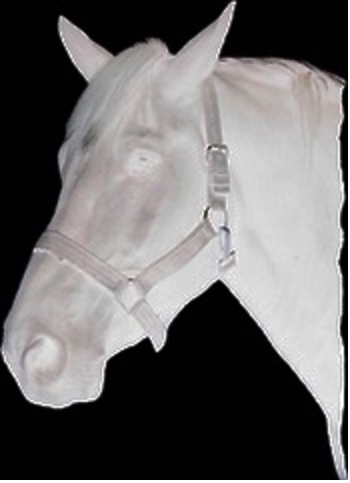
\includegraphics[width=0.6in]{Pictures/blackHorse.pdf}
\end{center}

\begin{figure}[t]
\begin{center}
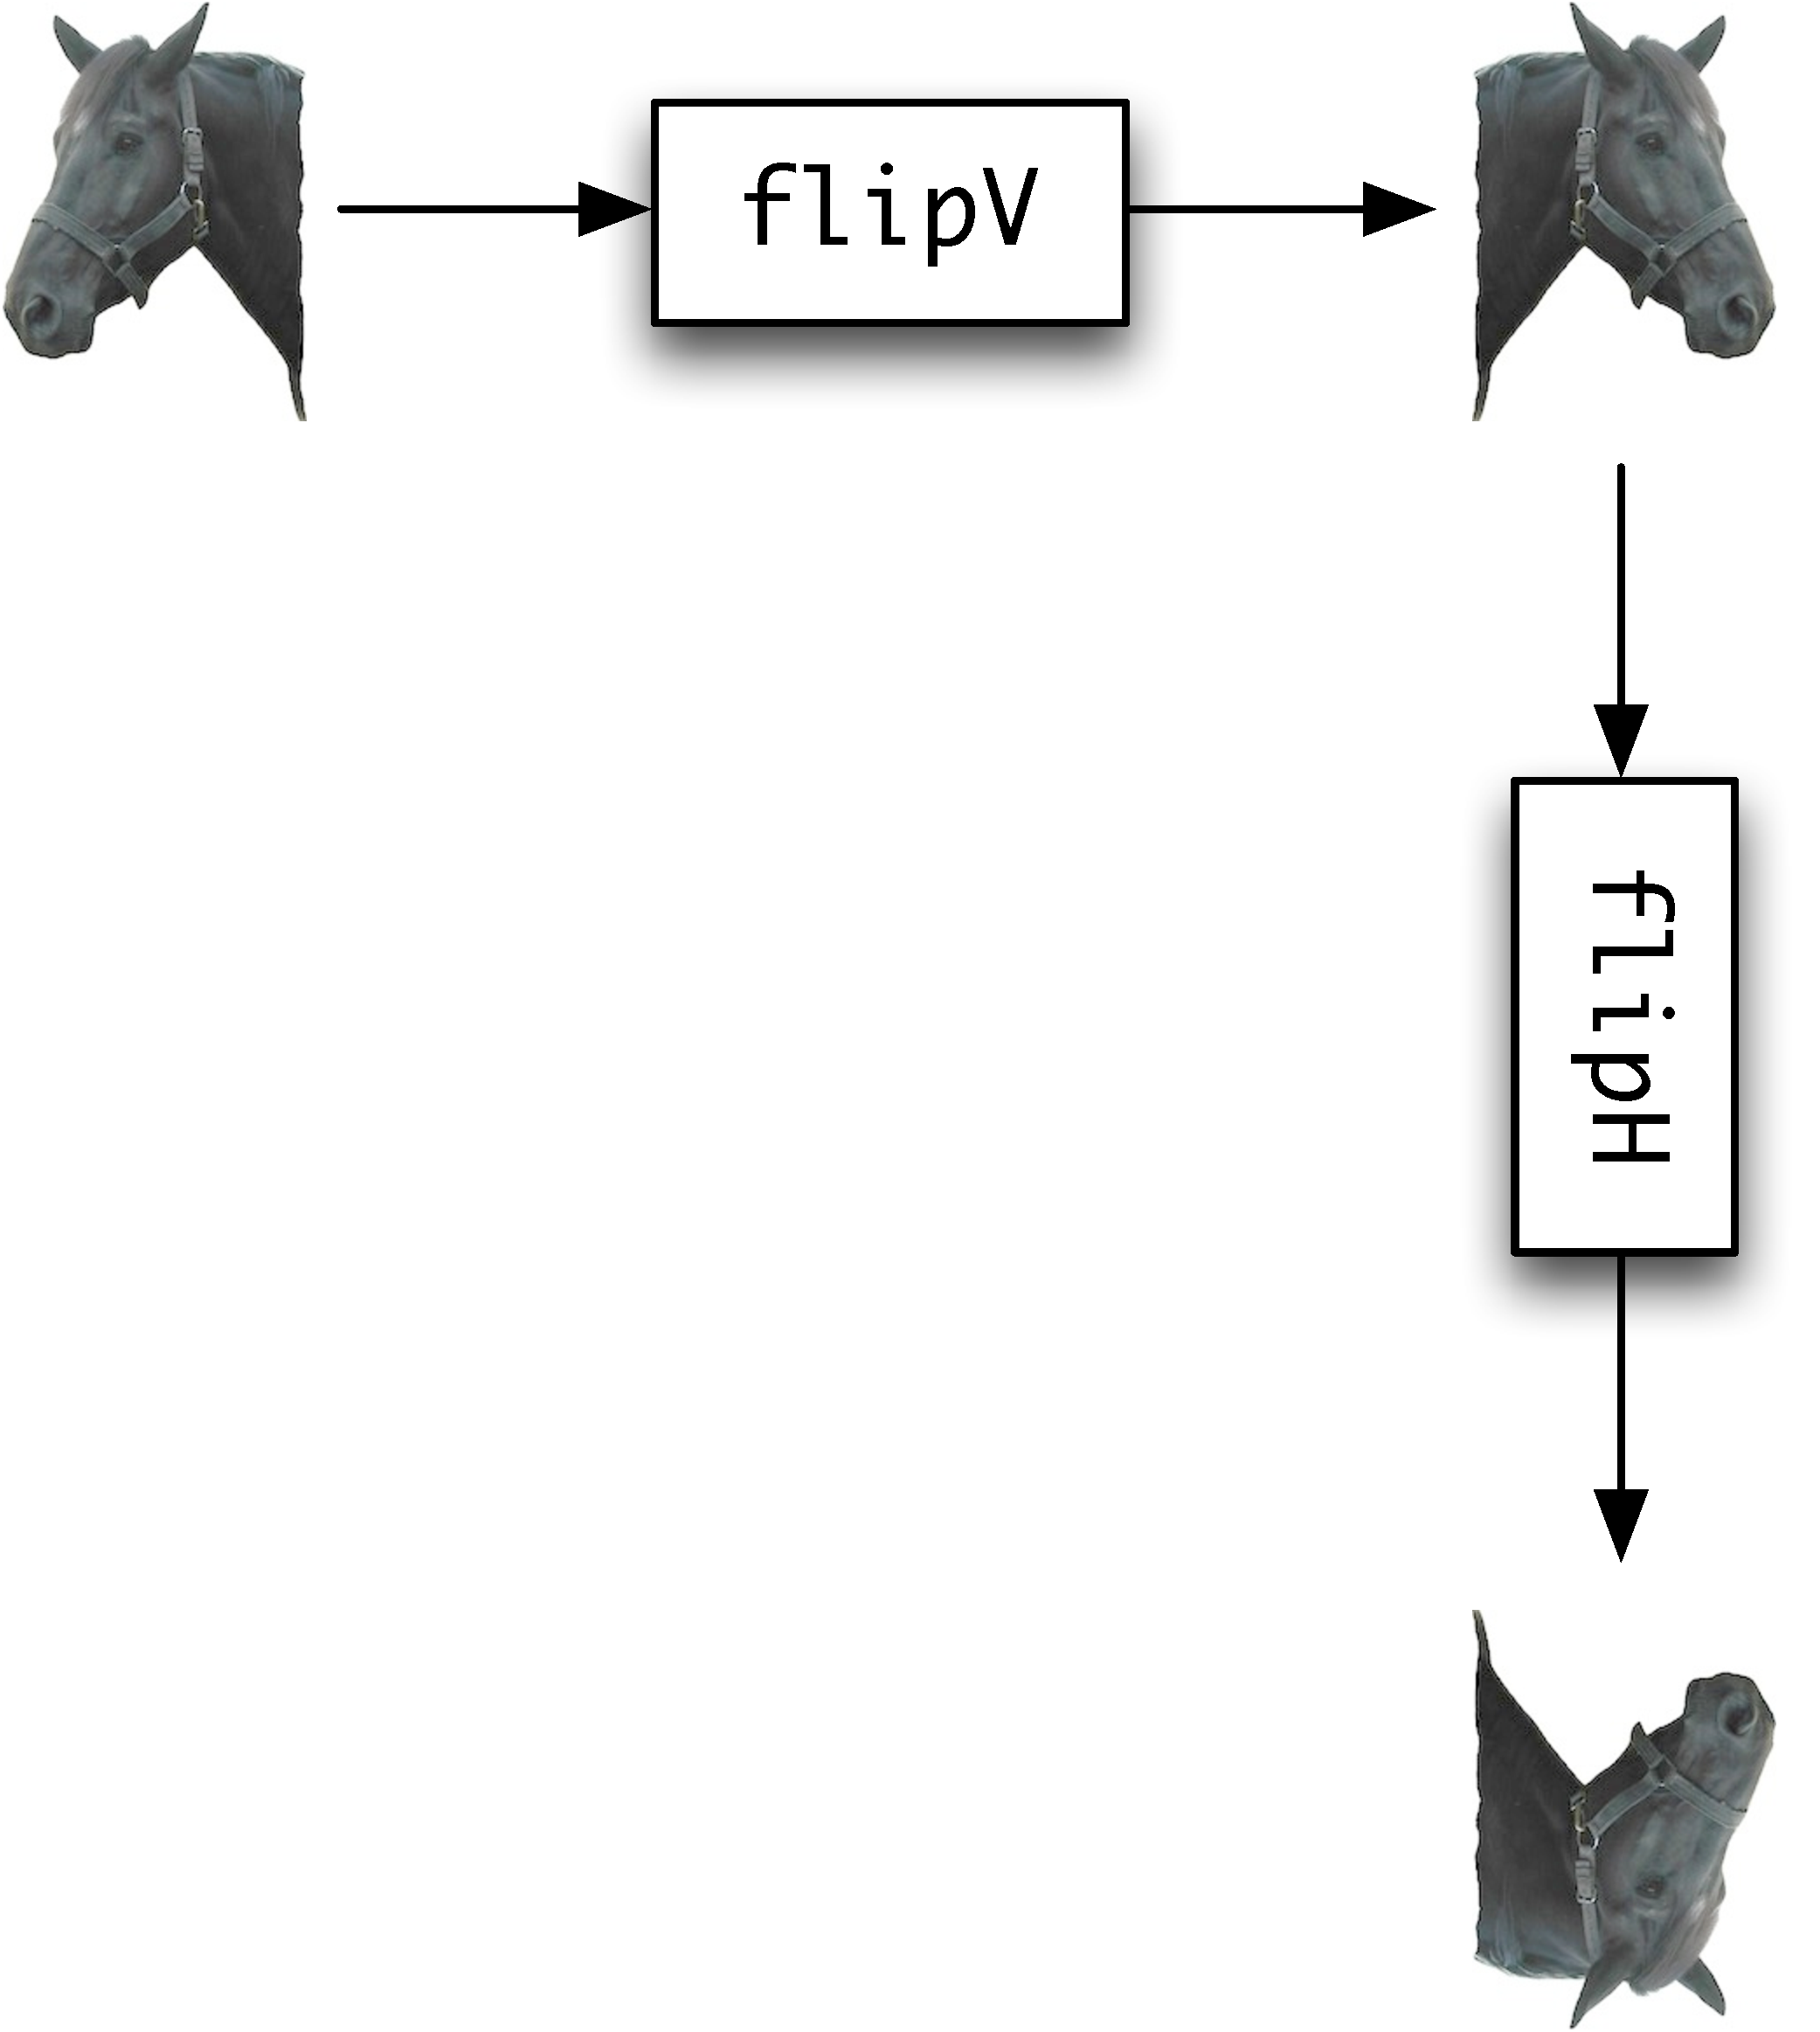
\includegraphics[width=3.0in]{Pictures/VthenH.pdf}
\end{center}
\caption{Calculating a rotation}
\label{flipping}
\end{figure}


\noindent
Another example is the definition
\begin{alltt}\minx{rotateHorse}
rotateHorse :: Picture
rotateHorse = flipH (flipV horse)
\end{alltt}
where Figure \ref{flipping} illustrates the evaluation of the right-hand side,
assuming that the function \texttt{flipH} has the effect of reflecting a
\texttt{Picture} in a horizontal mirror. The effect of these
two reflections is to rotate the picture through $180^\circ$.

In Section \ref{exprEval} we explained that GHCi works rather
like a calculator in evaluating expressions. How will it evaluate an
expression like
\begin{alltt}
size - 17
\end{alltt}
for instance?
Using the definition of \texttt{size} given earlier, we can replace the left-hand side 
-- \texttt{size} -- with 
the corresponding right-hand side -- \texttt{12+13}; this gives us the expression
\begin{alltt}
(12+13) - 17
\end{alltt}
and so by doing some arithmetic we can
see that the value of the expression is \texttt{8}.

The definitions we have seen so far are simply of constant values; we
now turn find out how functions are defined.

\section{Function definitions}
\label{funDefs}
\index{definition!function}
\index{function!definition}

We can also define functions, and we look at some simple examples now.
To square an integer we can say
\begin{alltt}
square :: Integer -> Integer\minx{square}
square n = n*n
\end{alltt}
where diagrammatically the definition is represented by
\begin{center}\minx{horse}\index{pictures!horse}
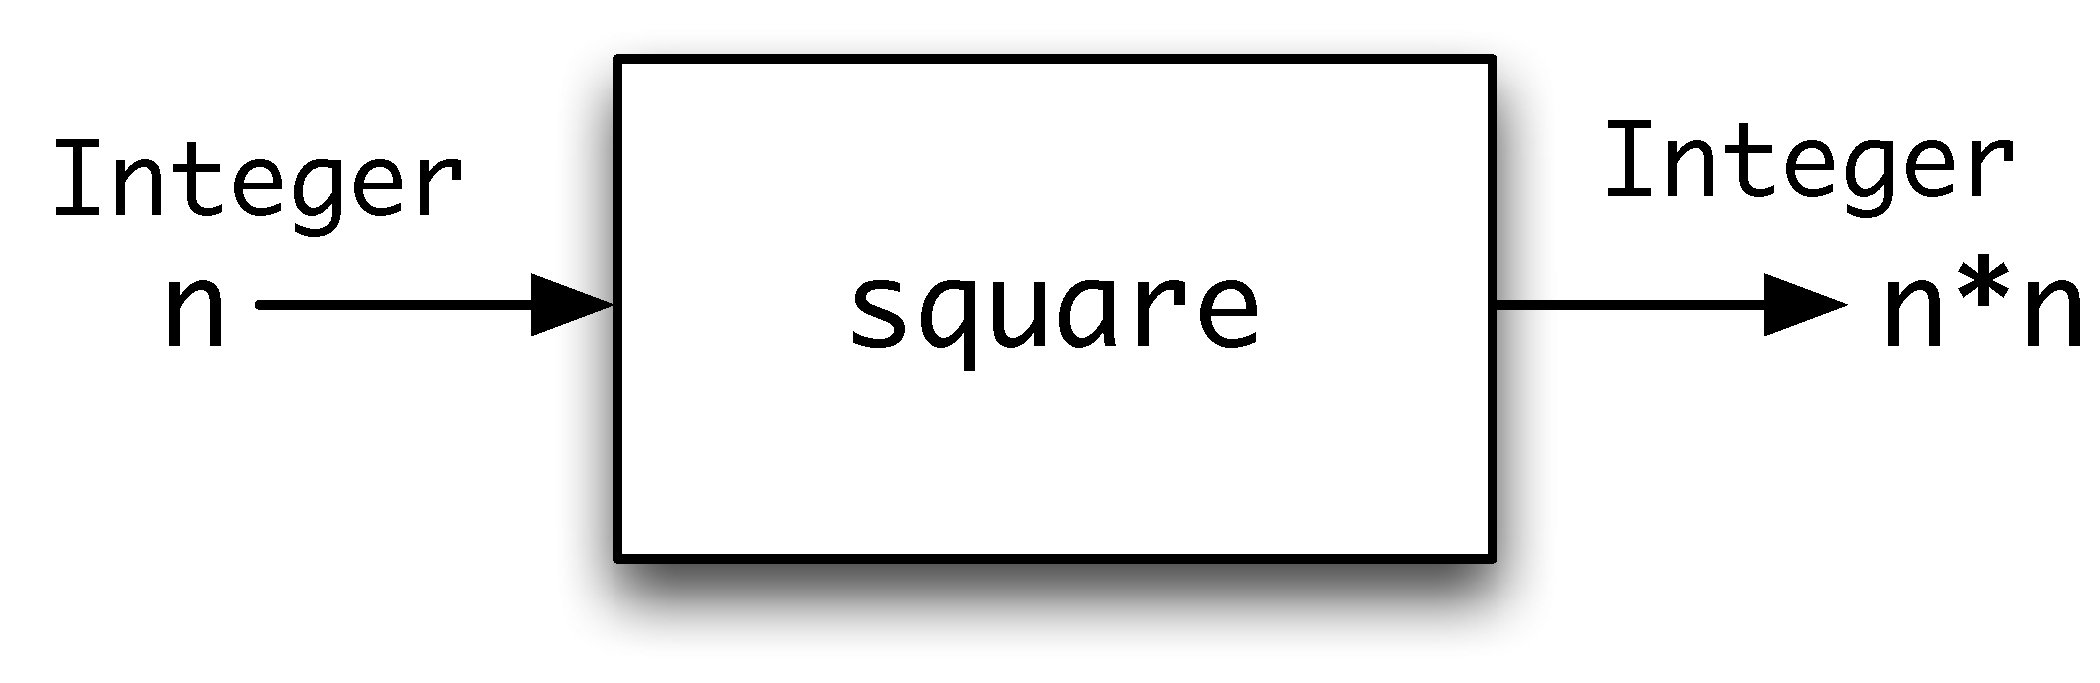
\includegraphics[width=3in]{Pictures/square.pdf}
\end{center}
The first line of the Haskell definition of \texttt{square}
declares the type of the thing being defined. The arrow \texttt{->} signifies that this is a function, with one input, an \texttt{Integer}, appearing before the arrow, and, coming after the arrow, a result of type
\texttt{Integer}. So, we can read \texttt{square ::\ Integer -> Integer} as 
\begin{quote}
``\texttt{square} is a function taking an \texttt{Integer} to an \texttt{Integer}''
\end{quote}\index{reading `\texttt{::}'}
The second line gives the definition of the function: the
equation\index{equation} says that when \texttt{square} is applied to an
\textbf{unknown}\index{unknown} or \textbf{variable}\index{variable}
\texttt{n}, then the result is \texttt{n*n}. How should we read an
equation like this? Because \texttt{n} is an arbitrary, or unknown value, it 
means that the equation holds {\em whatever the
value of\/} \texttt{n}, so that it will hold whatever integer expression we put
in the place of \texttt{n}, so that, for instance
\begin{alltt}
square 5 = 5*5
\end{alltt}
and
\begin{alltt}
square (2+4) = (2+4)*(2+4)
\end{alltt}
This is the way that the equation is used in evaluating an expression
which uses \texttt{square}. If we need to evaluate
\texttt{square} applied to the expression \texttt{e}, we replace the
application \texttt{square e} with the corresponding right-hand side,
\texttt{e*e}.

In general a simple function definition will take the form
\begin{center}\index{function definition!general case!single equation}
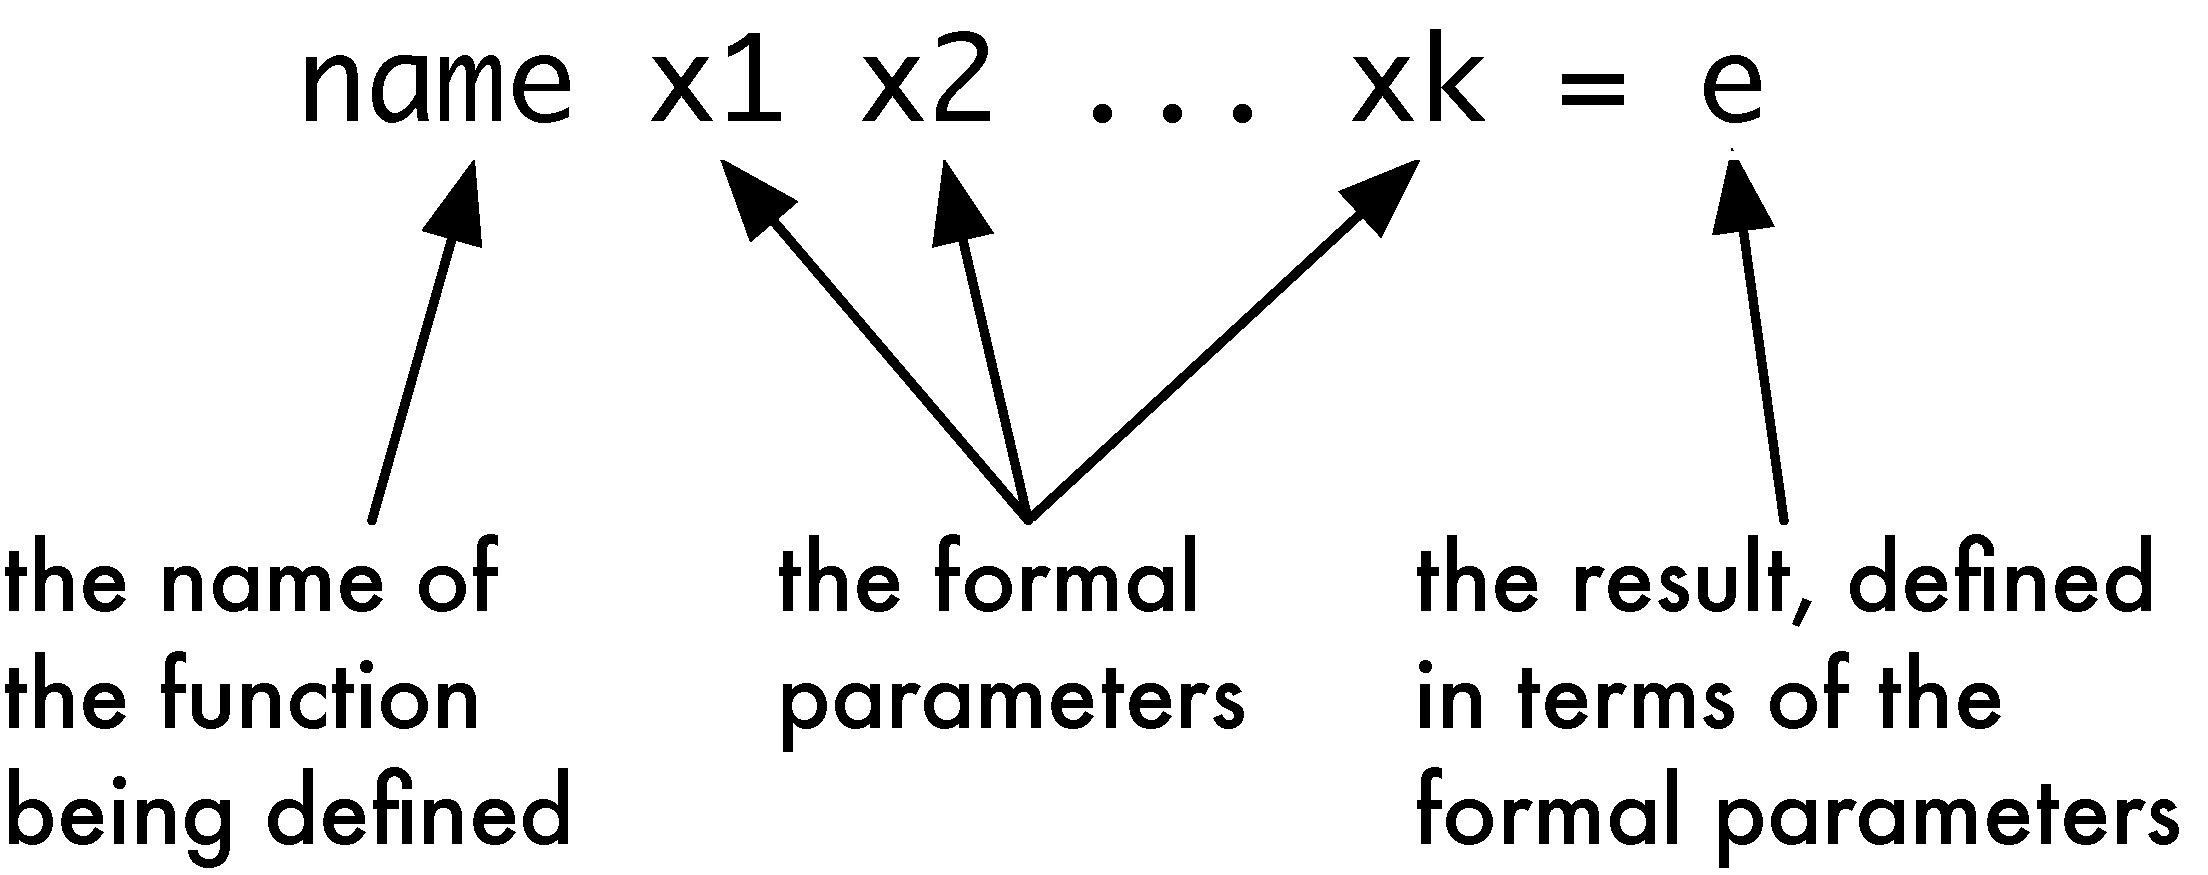
\includegraphics[width=3in]{Pictures/funDef.pdf}
\end{center}
The variables used in an equation defining a
function stand for arbitrary values: the definition holds for whatever value is chosen for these inputs. These variables are called the \textbf{formal parameters}\index{formal
parameter}\index{parameter!formal} of the function because they stand for arbitrary
values of the parameters: the \textbf{actual} parameters\index{actual
parameter}\index{parameter!actual} are supplied when the function is applied, as in \texttt{square 7}, where \texttt{7} is the actual parameter to \texttt{square}. We'll
only use `formal' and `actual' in the text when we need to draw a
distinction between the two; in most cases it will be obvious what is
meant when `parameter' is used.

Accompanying the definition of the function is a statement or \textbf{declaration}\index{type declaration} 
of its
type. That will look like this, using the \texttt{scale} function
over pictures as an example:
\begin{center}
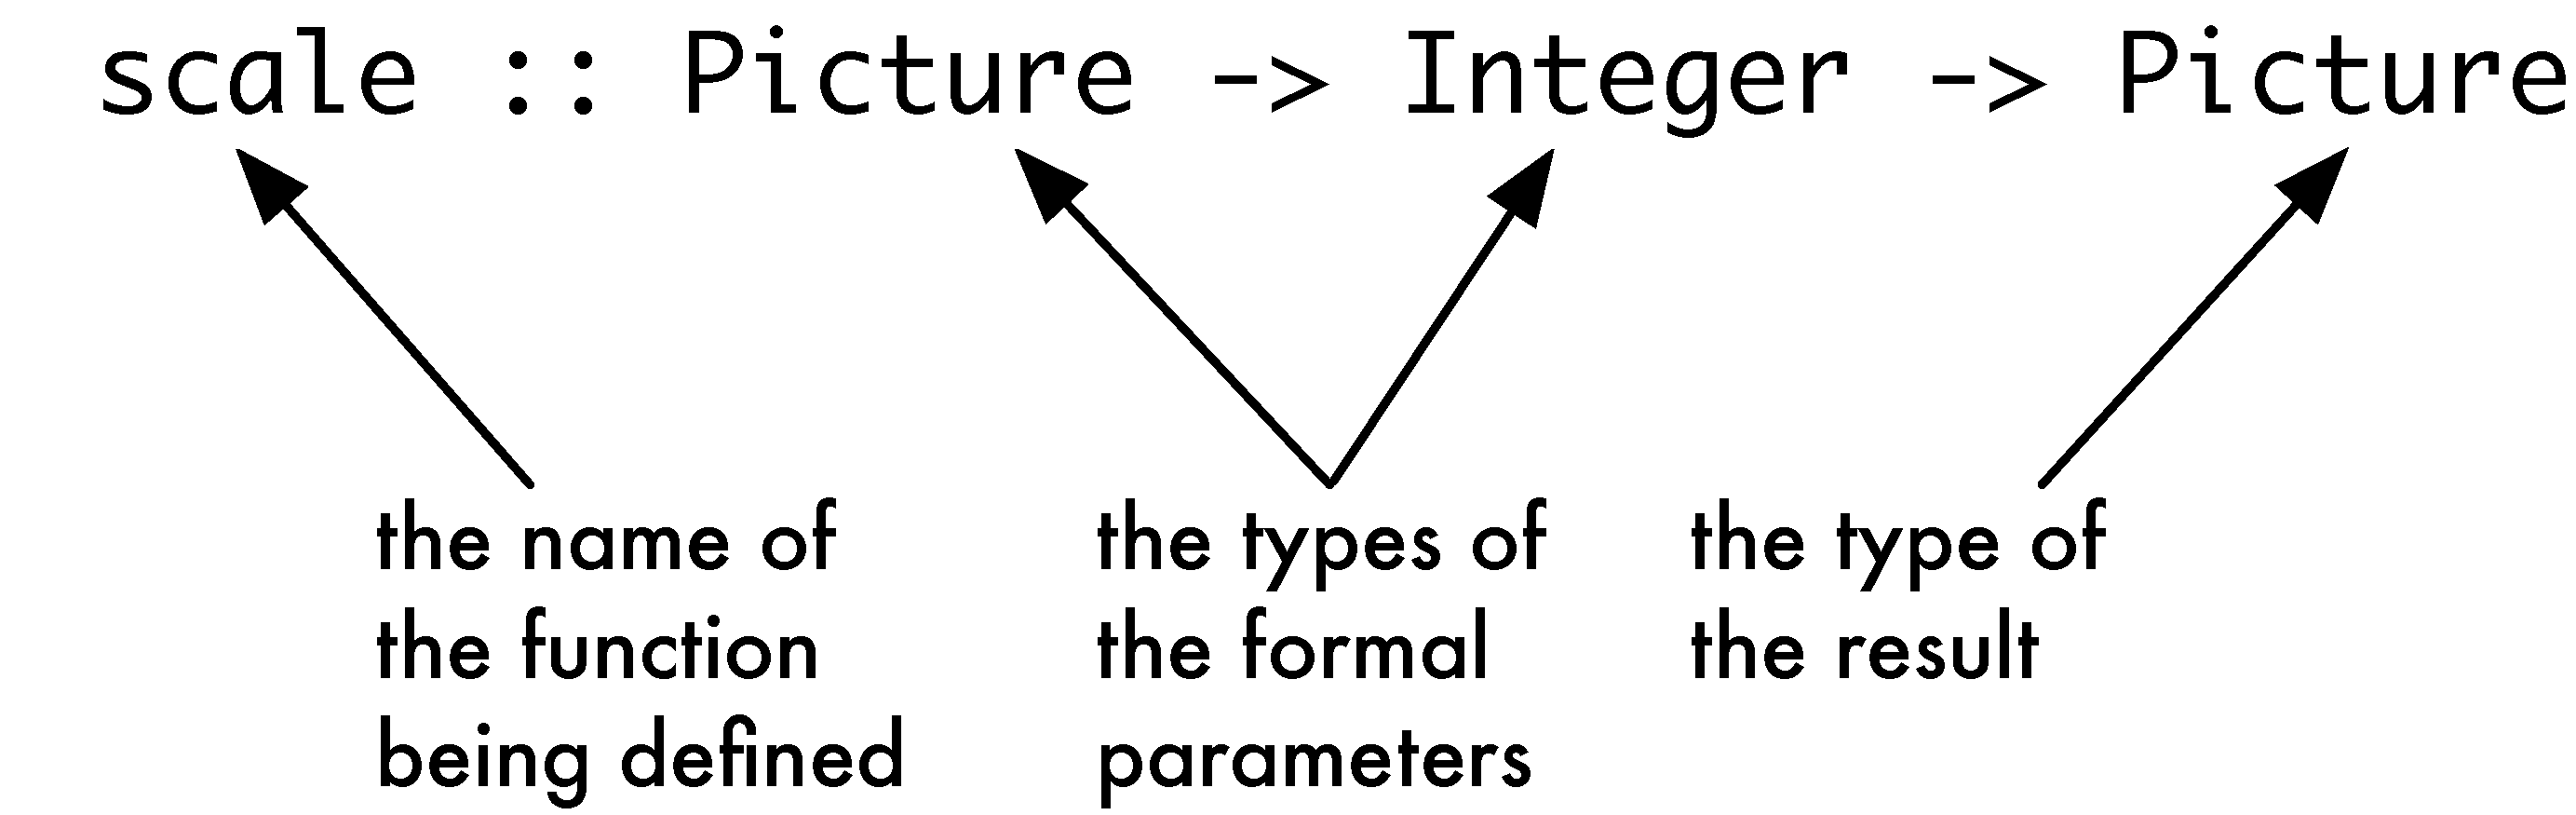
\includegraphics[width=4in]{Pictures/typeDiag.pdf}
\end{center}\index{scale@\texttt{scale}!type declaration}
In the general case we have
\begin{center}\index{type declaration!for function}
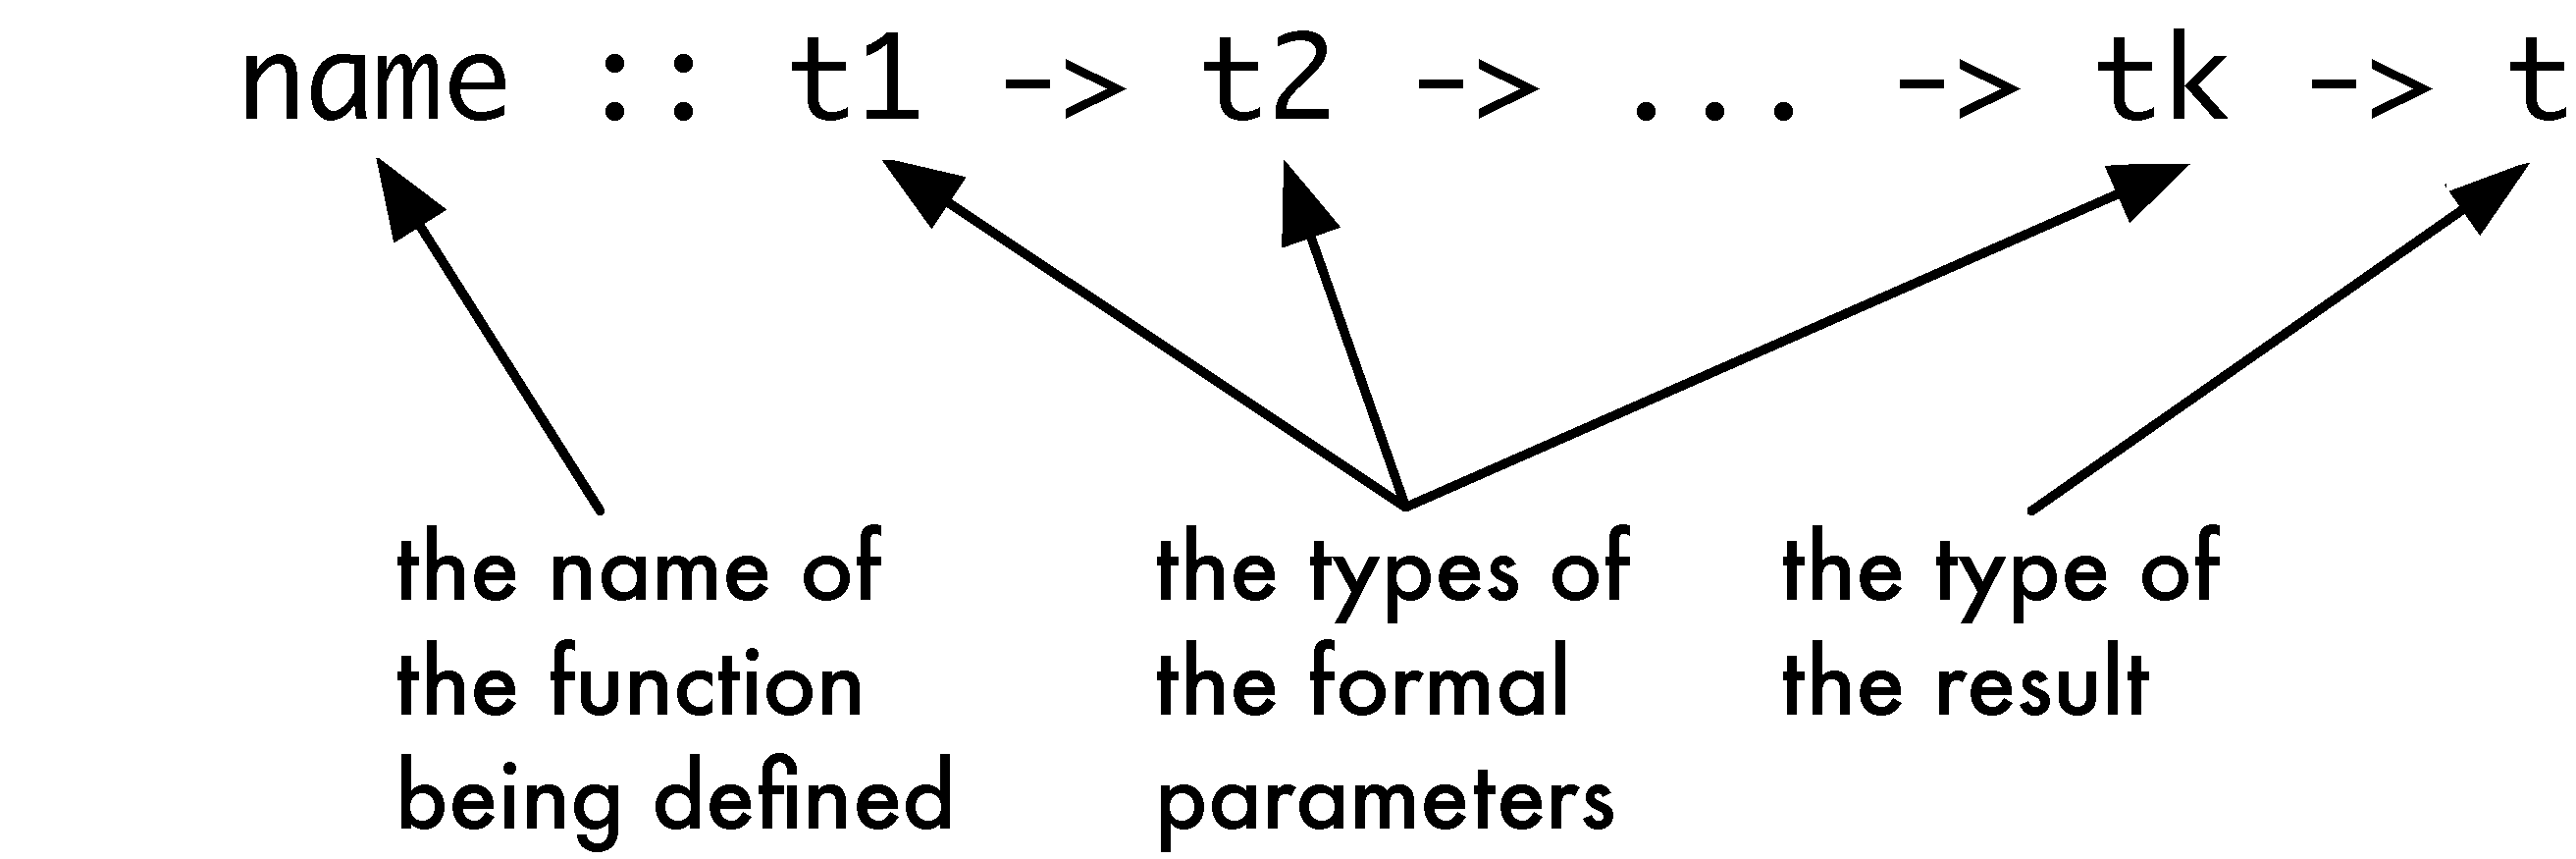
\includegraphics[width=4in]{Pictures/funTypeDef.pdf}
\end{center}
The definition of \texttt{rotateHorse} in Section \ref{defsIntro}
suggests a general definition of a rotation function. To
rotate {\em any\/} picture we can perform the two reflections, and so we
define
\begin{alltt}
rotate :: Picture -> Picture
rotate pic = flipH (flipV pic)
\end{alltt}
We can read the definition like this:
\begin{quote}
To \texttt{rotate} a picture \texttt{pic}, we first apply \texttt{flipV}
to form \texttt{(flipV pic)}; we then apply \texttt{flipH} to reflect this in a horizontal mirror, giving the result \texttt{flipH (flipV pic)}.
\end{quote}
Given this definition, we can replace the definition of
\texttt{rotateHorse} by
\begin{alltt}
rotateHorse :: Picture
rotateHorse = rotate horse
\end{alltt}
which states that \texttt{rotateHorse} is the result of applying the
function \texttt{rotate} to the picture \texttt{horse}.

The pattern of definition of \texttt{rotate} -- `apply one function, and
then apply another to the result' -- is so common that Haskell gives a
way of combining 
functions directly in this way. We define
\begin{alltt}\minx{rotate}
rotate :: Picture -> Picture
rotate = flipH . flipV
\end{alltt}\label{here}
The `\texttt{.}'\minx{.} in the definition signifies \textbf{function
composition}\index{function composition}\index{composition|see{function composition}}, in which
the output of one function becomes the input of another. In pictures, 
\begin{center}
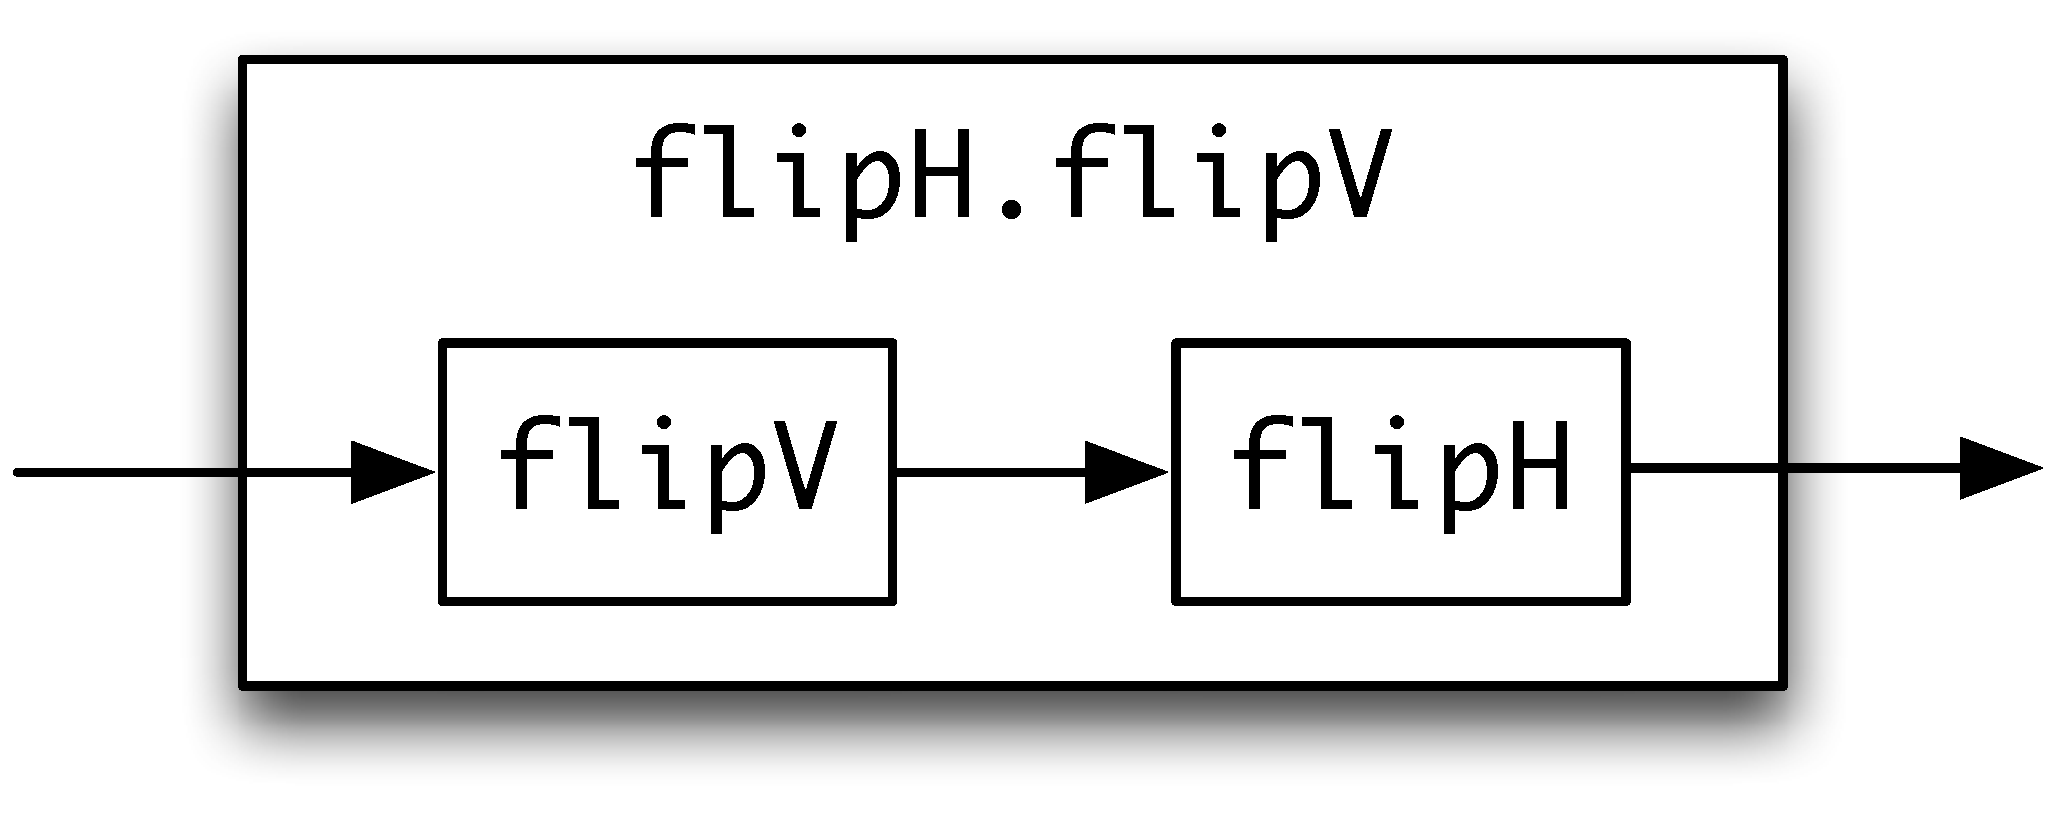
\includegraphics[width=3in]{Pictures/HVcompos.pdf}
\end{center}
we see the creation of a new function by connecting together the input
and output of two given functions: obviously this suggests many other
ways of connecting together functions, many of which we will look at in
the chapters to come.

The direct combination of functions is one example of the
power of functional programming: we are able to combine functions using
an operator like `\texttt{.}' just as we can combine
numbers using `\texttt{+}'. We use the term `\textbf{operator}'\index{operator} here
rather than `function' since `\texttt{.}' is written between its
arguments rather than before them; we discuss operators in more detail
in Section \ref{syntax}.

The direct combination of functions by means of the operator `\texttt{.}'
which we have seen here 
is not possible in other programming
paradigms, or at least it would be an `advanced' aspect of the language,
rather than appearing on page \pageref{here} of an
introductory text.



\section{Types and functional programming}
\label{typesFP}
\index{type!importance of types}

What is the role of types in functional programming? Giving a type to a
function first of all gives us crucial information about how it is to be
used. If we know that
\begin{alltt}
scale :: Picture -> Integer -> Picture
\end{alltt}\index{scale@\texttt{scale}!type declaration}\index{type declaration!understanding}
we know two things immediately.
\begin{itemize}
\item First, \texttt{scale} has two arguments: the first is a
\texttt{Picture} and the second an \texttt{Integer}; this means that
\texttt{scale} can be applied to \texttt{horse} and \texttt{3}.
\item The result of applying \texttt{scale} to this \texttt{Picture} and \texttt{Integer}
will be a \texttt{Picture}.
\end{itemize}
The type thus does two things. First, it expresses a
\textbf{constraint}\index{constraint}\index{type!constraint} on how the
function \texttt{scale} is applied: it must be applied 
to a \texttt{Picture} and an \texttt{Integer}. Second, the type tells us
what the result is if the function is correctly applied: in this case
the result is a \texttt{Picture}.

Giving types to functions and other things not only tells us how they
can be used; it is also possible to check automatically that functions
are being used in the right way and this process -- which is called
\textbf{type checking}\index{type checking} -- takes place in Haskell. If we
use an expression like 
\begin{alltt}
scale horse horse
\end{alltt}
we will be told that we have made an error in applying \texttt{scale} to
two pictures
when a picture and a number are what was expected. Moreover, this can be done without knowing
the {\em values\/} of \texttt{scale} or \texttt{horse} -- all that we need to know 
to perform the check is the {\em types\/} of the things concerned.
Thus, \textbf{type errors}\index{type error} like these 
are caught before programs are used or expressions
are evaluated.

It is remarkable how
many errors, due either to mistyping or to misunderstanding the problem, are made
by novices and experienced programmers alike.  The Haskell type system
therefore helps us to write correct programs, and to avoid a large proportion 
of programming pitfalls, both 
obvious and subtle, typos and misunderstandings. This is something which you particularly appreciate if you do use other languages without this kind of type checking, where you need to trace back from a particular error that happens during evaluation to its source.

\subsection*{Type abstraction}
\index{abstraction!type}\index{type!abstract}

Before moving on, there is another important point which we'll
explore later in the book. In Sections \ref{defsIntro} and \ref{funDefs}
we gave definitions of
\begin{alltt}\minx{Picture}\minx{rotate}
blackHorse :: Picture
rotate     :: Picture -> Picture
\end{alltt}
which \textbf{use} the type \texttt{Picture} and some functions already defined
over it: \texttt{flipH} and \texttt{flipV}. We were able to
write the definitions of
\texttt{blackHorse} and \texttt{rotate} {\em without
knowing anything about\/} how the type of \texttt{Picture}s or the functions working with \texttt{Picture}s were actually defined. We can use these functions because we know their types, so we know what they have to be applied to, and what type their results will be.

Treating the type \texttt{Picture} in this way is called
\textbf{type abstraction}:
as users of the type we don't need to concern ourselves with how the type is
defined. The advantage of this is that the definitions we give apply {\em
however\/} pictures are modelled. We might choose to model them in
different ways in different situations; whatever the case, the function
composition
\texttt{flipH .\ flipV} will rotate a
picture through $180^\circ$. We'll see this in practice in Section \ref{two-models} where we give two, very different, models of pictures; 
Chapter \ref{adt} discusses this in more
detail, and explains the Haskell mechanism to support type abstraction.



\section{Calculation and evaluation}
\index{calculation}\index{evaluation}

We have explained that GHCi can be seen as a general calculator, using
the functions and other things defined in a functional program. When we
evaluate an expression like
\begin{alltt}
23 - (double (3+1))\hfill(\ddag)
\end{alltt} 
we need to use the definition of the function:
\begin{alltt}
double :: Integer -> Integer
double n = 2*n\hfill(dbl)
\end{alltt}\minx{double}
This we do by replacing the unknown \texttt{n} in the definition
\texttt{(dbl)} by the
expression \texttt{(3+1)}, giving 
\begin{alltt}
double (3+1) = 2*(3+1)
\end{alltt}
Now we can replace \texttt{double (3+1)} by \texttt{2*(3+1)} in \texttt{(\ddag)}, and
evaluation can continue.

One of the distinctive aspects of functional programming is that such a
simple 
`calculator' model is a complete description of computation in Haskell. Because the model is so straightforward, we can perform
evaluations in a \textbf{step-by-step}\index{evaluation!step-by-step}
manner; in this text we call these step-by-step evaluations
\textbf{calculations}\index{calculation}.
As an example, we now show the calculation of the expression with which we 
began the discussion.
\begin{alltt}
23 - (double (3+1))
\step 23 - (2*(3+1))\hfill\textrm{using} \texttt{(dbl)}
\step 23 - (2*4) \hfill\textrm{arithmetic}
\step 23 - 8 \hfill\textrm{arithmetic}
\step 15 \hfill\textrm{arithmetic}
\end{alltt}
where we have used `\step'\index{\step} to indicate a step of the calculation, and on
each line we indicate at the right-hand margin how we have reached that
line. For instance, the second line of the calculation:
\begin{alltt}
\step 23 - (2*(3+1))\hfill\textrm{using} \texttt{(dbl)}
\end{alltt}
says that we have reached here using the definition of the
\texttt{double} function, \texttt{(dbl)}.

In writing a calculation it is sometimes useful to \underline{underline}\index{underlining@\underline{underlining}}
the part of the expression which gets modified in transition to the next
line. This is, as it were, where we need to focus our attention in
reading the calculation. The calculation above will have underlining
added like this:
\begin{alltt}
23 - \underline{(double (3+1))}
\step 23 - (2*\underline{(3+1)})\hfill\textrm{using} \texttt{(dbl)}
\step 23 - \underline{(2*4)} \hfill\textrm{arithmetic}
\step \underline{23 - 8} \hfill\textrm{arithmetic}
\step 15 \hfill\textrm{arithmetic}
\end{alltt}
In what is to come, when we introduce a new feature of Haskell we shall
show how it fits into this line-by-line model of evaluation. This has
the advantage that we can then explore new ideas by writing down
calculations which involve these ideas.


\section{The essence of Haskell programming}
\index{programming paradigms!comparison}

We've learned enough about functional programming in Haskell to compare it with other kinds of programming paradigm, particularly OO and other imperative languages. First we'll summarise the essentials of Haskell, and then look at how it differs from others approaches.

So, what makes functional programming in Haskell special? Working in Haskell we concentrate on using a rich collection of data types -- including functions themselves, as well as types defined by the user -- to model the objects in the problem domain. Programming over these is done by writing functions: functions are defined by equations like
\begin{alltt}
rotate :: Picture -> Picture
rotate pic = flipH (flipV pic)\hfill\texttt{(rotate)}
\end{alltt}
Finally, computing with these functions is done by calculation, or evaluation, using the definitions to calculate a result as we saw in the last section. In a equation like \texttt{(rotate)}, \texttt{pic} is a variable, in the mathematical sense of something that stands for an \emph{arbitrary} \texttt{Picture}.

If you know Java, or another OO or imperative language like C, C++ or C\#, then you need to understand that Haskell variables are very different from variables in these languages. A Java variable is like a box, where values can be stored: the value is changed by making an assignment. In Java we compute by changing these contents, or the\texttt{state} as it is called. Methods which change state are said to have \textbf{side-effects}\index{side-effect}. 

By contrast, Haskell variables don't vary, and the way we program is to write functions which describe how particular data values are related. These functions don't have side-effects, and there is no state in Haskell. We'll find about how all of this works in the chapters to come, we can summarize the important advantages now.
\begin{itemize}
\item
Haskell programs are \emph{higher-level}: they can be read as a direct description of \emph{what} are the relationships between input and output data, rather than covering the details of \emph{how} a result is computed in a series of steps that change the values of variables.
\item
Functions in Haskell can themselves be passed around just like any other \emph{data}. So, we can use functions as well as all the other Haskell types when we're modelling complex problems.
\item
Haskell functions are without side-effects, but in Haskell it's possible to do I/O, work with files, and inter-operate with other programming languages. We can do this using \emph{monads} which allow these `computational effects' to be embedded inside Haskell and its type system.
\item
Haskell programs are easy to \emph{parallelise}, and to run efficiently on multicore hardware, because there is no state to be shared between different threads. In Java different treads share the same state, and it's very hard to make sure that a Java program will run efficiently -- or even correctly -- in a multicore environment.
\item
If definitions are equations, then it's possible to think of them as expressing \emph{properties} of programs, and we can use these to write \emph{proofs} of other properties our programs have, and so validate what they do.
\item
There are often many different ways of solving the same problem, and when we begin to try to solve a problem it can be very hard to know which approach to take. Because Haskell programs are free of side-effects it's much easier to transform or \emph{refactor} our programs to have a different design, as we might need to do before extending or modifying our program.
\end{itemize} 
Taking these together, we can see why Haskell is popular for many tasks, and particularly for writing domain-specific languages, which we look at now.


\section{Domain-specific languages}
\index{domain-specific language|see{DSL}}\index{DSL|(} 

Haskell is a general-purpose programming language: it can be used to solve any kind of programming problem. Other languages, called \textbf{domain-specific languages} (\textbf{DSLs}) or \textbf{little languages}, are designed to solve problems in a particular domain. For example, this book has been written using \LaTeX, a language for typesetting; other DSls are used for hardware design (Verilog), statistics (R, Excel) and graph layout (GraphViz).
Stand-alone DSLs like these have the advantage that everything about them, from the way that programs are written to the details of what they mean, can be adapted to the particular domain. On the other hand, all the infrastructure has to be built from scratch.

A different approach is not to build the DSL from scratch, but instead to embed it in an existing programming language. These \textbf{embedded domain-specific languages}\index{DSL!embedded} can take advantage of everything that the programming language provides, while expressing the concepts of the particular domain as well. Haskell has been particularly successful as a basis for embedding DSLs, including Lava \cite{lava} for circuit simulation and layout, Paradise \cite{paradise} for pricing financial products and Orc \cite{orc} for orchestrating scientific computations.

Why has Haskell been particularly successful for embedding DSLs? The rich set of data types -- including functions and user-defined \texttt{data} types -- which can be used to model the underlying domains; the absence of side-effects makes it possible to write models which focus on the data, independent of any state. More advanced aspects of Haskell also help the DSL writer. Some are beyond the scope of this text, but we'll cover three important features. Polymorphism and type classes are two different mechanisms to make it possible for functions to be used over multiple types: this allows a DSL to be interpreted in different ways; for example, this allows a hardware DSL can be used both for simulation and layout of circuits. Monads allow DSLs to have side-effects in a controlled way. We'll come back to this discussion as we look at DSLs in Haskell in Chapter \ref{dsls}.
\index{DSL|)} 


\begin{figure}[t]
\begin{center}
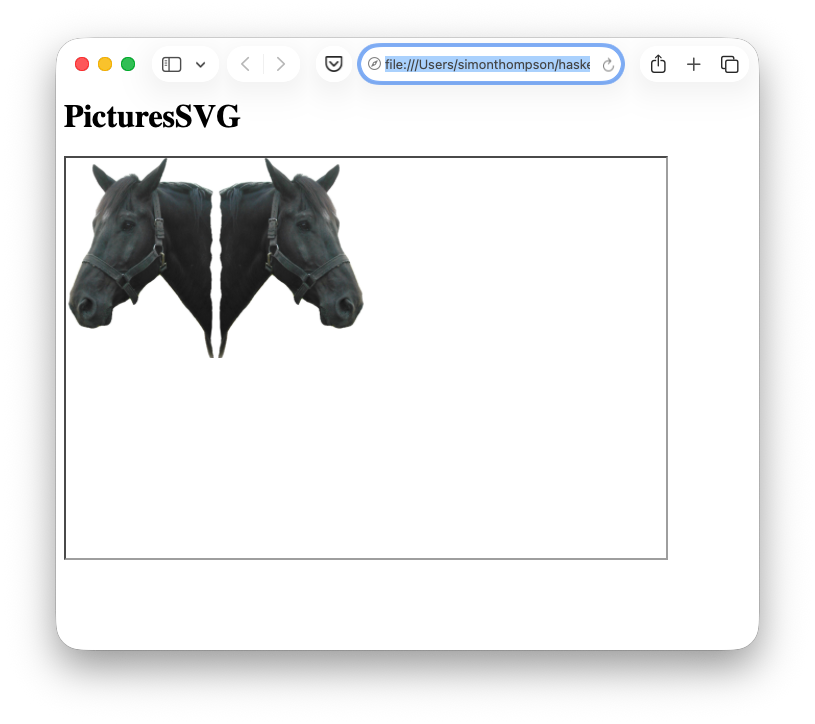
\includegraphics[width=\textwidth]{Pictures/ScreenSVG.png}
\end{center}
\caption{Viewing \texttt{Pictures} in a web browser}
\label{svgpix}
\end{figure}



\section{Two models of \texttt{Picture}s}
\label{two-models}
\index{pictures|(}\index{DSL!pictures}


This section looks at the pictures example as a small DSL, and gives two models -- or implementations -- of the pictures DSL.

\subsection*{The \texttt{Picture} DSL}

We can describe the DSL for \texttt{Picture}s by giving the type declarations of its constructs.
\begin{alltt}
horse        :: Picture

flipH        :: Picture -> Picture
flipV        :: Picture -> Picture
invertColour :: Picture -> Picture

above        :: Picture -> Picture -> Picture
beside       :: Picture -> Picture -> Picture

scale        :: Picture -> Integer -> Picture
\end{alltt}
We form complex pictures by combining these into expressions, such as
\begin{alltt}
horse `above` (flipH horse)
\end{alltt}
but because the DSL is embedded in Haskell we can use all the facilities of Haskell too.  We might make a complicated calculation of how much we want to scale a picture,
\begin{alltt}
scale (horse `above` (flipH horse)) (complicated Integer calculation)
\end{alltt}
but we can also use the facilities of Haskell for naming \texttt{Picture}s 
\begin{alltt}
bigPic = scale (horse `above` (flipH horse)) 42
\end{alltt}
and defining other functions
\begin{alltt}
mirror pic = pic `beside` (flipV pic)
\end{alltt}


\begin{figure}[t]
\begin{center}
\begin{alltt} 
.......##...               ......##....               ...##.......
.....##..#..               .....#.#....               ..#..##.....
...##.....#.               ....#..#....               .#.....##...
..#.......#.               ...#...#....               .#.......#..
..#...#...#.               ..#...#.....               .#...#...#..
..#...###.#.               .#....#..##.               .#.###...#..
.#....#..##.               ..#...###.#.               .##..#....#.
..#...#.....               ..#...#...#.               .....#...#..
...#...#....               ..#.......#.               ....#...#...
....#..#....               ...##.....#.               ....#..#....
.....#.#....               .....##..#..               ....#.#.....
......##....               .......##...               ....##......

horse                      flipH horse                flipV horse
\end{alltt}
\end{center}
\caption{ASCII-art pictures}
\label{Horses}\minx{horse}
\end{figure}


\subsection*{SVG pictures}

The pictures we've seen so far in this chapter are from a model of pictures which can be displayed in web browsers supporting the SVG standard\cite{SVG},\index{SVG} as shown in Figure \ref{svgpix}. The web page allows you to view pictures ``rendered from'' Haskell descriptions; we'll come back to the details of how this is done in Section \ref{ShowBrowser}, page \pageref{ShowBrowser}. For now the message is that you can use the DSL just knowing the types of the functions, as they tell you all you need to know to use them: for each function they tell us the types of the inputs they should be applied to and the type of the result.

\subsection*{Pictures and lists}


We include this section in the first chapter of the book for two reasons.
To start with, we want to describe a second way in which \texttt{Picture}s can be 
modelled in Haskell. 
Secondly, we want to provide an
informal preview of a number of aspects of Haskell which make it
a powerful and distinctive
programming tool. As we go along we will indicate
the parts of the book where we expand on
the topics first introduced here.

Our model consists of two-dimensional, monochrome pictures built 
from \textbf{characters}\index{characters}.
Characters are the individual letters,
digits, spaces and so forth which can be typed at the computer keyboard and which 
can also be shown on a computer screen. In Haskell the characters are
given by the built-in type
\texttt{Char}\minx{Char}. 
This model has the advantage that it is straightforward to view these
pictures on a computer terminal window. 


Our version of the \texttt{horse} picture, and the same picture
flipped in horizontal and vertical mirrors are shown in Figure \ref{Horses},
where we use dots to show the white parts of the pictures.

How are the pictures built from characters? In our model we think of
a picture as being made up of
a \textbf{list}\index{lists} of lines, that is a collection of
lines coming one after another in order. Each line can be seen in a similar way
as a list of characters. Because we often deal with collections of things when programming, 
lists are built into Haskell. More specifically, given any type -- like characters or lines
-- Haskell contains a type of lists of that type, and so in particular we can model pictures
as we have already explained, using lists of characters
to represent lines, and lists of lines to represent pictures.

With this model of \texttt{Picture}s, we can begin to think about how to
model functions over pictures. A first definition comes easily; to
reflect a picture in a horizontal mirror each line is unchanged, but
the order of the lines is reversed: in other words we reverse the list
of lines:
\begin{alltt}
flipH = reverse\minx{flipH}\minx{reverse}
\end{alltt}
where \texttt{reverse} is a built-in function to reverse the order of items
in a list.
How do we reflect a picture in a vertical mirror? The ordering of the
lines is not affected, but instead {\em each line is to be reversed}. We can write
\begin{alltt}
flipV = map reverse\minx{flipV}
\end{alltt}
since \texttt{map}\index{map@\texttt{map}} is the Haskell function which applies a function
to each of the items in a list, individually.
In the definitions of \texttt{flipH} and \texttt{flipV} we can begin to see the power 
and elegance of
functional programming in Haskell.
\begin{itemize}
\item 
We have used \texttt{reverse} to reverse a list of lines in
\texttt{flipH} and to reverse each line in \texttt{flipV}: this is
because the same
definition of the function \texttt{reverse} can be used over {\em every\/}
type of list. This is an example of polymorphism,\index{polymorphism} or generic
programming, which is examined in detail in Section \ref{poly}.
\item 
In defining \texttt{flipV} we see the function \texttt{map}
applied to its argument \texttt{reverse}, {\em which is itself a
function}. This makes \texttt{map} a very general function, as it can have
any desired action on the elements of the list, specified by the function
which is its argument. This is the topic of Chapter \ref{patternsGen}.
\item 
Finally, the {\em result\/} of applying \texttt{map} to
\texttt{reverse} is itself a function. This covered in Chapter \ref{gen2}.
\end{itemize}
The last two facts show that functions are `first-class citizens'
\index{first-class citizens, functions} 
\index{function!first-class citizens}
and
can be handled in exactly the same way as any other sort of object like
numbers or pictures. The combination of this with polymorphism means
that in a functional language we can write very general functions like
\texttt{reverse} and \texttt{map}, which can be applied in a multitude of
different situations.

The examples we have looked at here are not out of the ordinary. We can see that
other functions over pictures have similarly simple definitions. We
place one picture \texttt{above} another simply by joining together the two 
lists of lines to make one list. This is done by the built-in operator
\texttt{++}\minx{++},
which joins together two lists:\footnote{The operator \texttt{++} is
surrounded by parentheses \texttt{(...)} in this definition so that it
is interpreted as a function; we say more about this in 
Section \ref{syntax}\index{operator!as function}.}
\begin{alltt}
above = (++)\minx{above}
\end{alltt}

To place two pictures \texttt{beside} each other we have to join corresponding
lines together, thus
\begin{alltt}\label{beside}\minx{beside}
.......##...   ++   ......##....
.....##..#..   ++   .....#.#....
...##.....#.   ++   ....#..#.... 
..#.......#.   ++   ...#...#.... 
..#...#...#.   ++   ..#...#.....
..#...###.#.   ++   .#....#..##.    
.#....#..##.   ++   ..#...###.#.    
..#...#.....   ++   ..#...#...#.     
...#...#....   ++   ..#.......#.     
....#..#....   ++   ...##.....#.      
.....#.#....   ++   .....##..#..      
......##....   ++   .......##...         
\end{alltt}
and this is defined using the function \texttt{zipWith}. This function is
defined to `zip together' corresponding elements of two lists
using -- in this case -- the operator \texttt{++}.
\begin{alltt}\index{zipWith@\texttt{zipWith}}
beside = zipWith (++) 
\end{alltt}
We shall return to these examples in Chapter \ref{gen2}.
\index{pictures|)}


\section{Tests, properties and proofs}
\label{proof}\label{pictureProps}



\noindent
How can we be sure that a program we have written does what it should? The traditional answer is to test the program on a selection of inputs, and of course we can -- and should -- do this for Haskell programs. We've got two other more powerful options, \textbf{property-based testing}\index{property-based testing}\index{testing!property-based} and \textbf{proof}, and we'll introduce those in this section, and follow them up in the rest of the book. 

\subsection*{Tests and properties}

Let's look at the example of \texttt{Picture}s from the last section: how do we test this? One way of doing this is to write tests of the form:
\begin{quote}
``apply this function to this input \ldots the output should be this''
\end{quote}
Given the picture library, we can also look at how the functions work together, and a  simple way of doing this is to check how a combination of applications works. For example, 
\begin{itemize}
\item
if we flip a picture twice in a mirror we should get back the original picture;
\item
if we flip a picture in both a horizontal and vertical mirror, it shouldn't matter the order in which we do this, as illustrated in Figure \ref{vh-hv}, page \pageref{vh-hv}.  
\end{itemize}
\begin{figure}[t]
\begin{center}
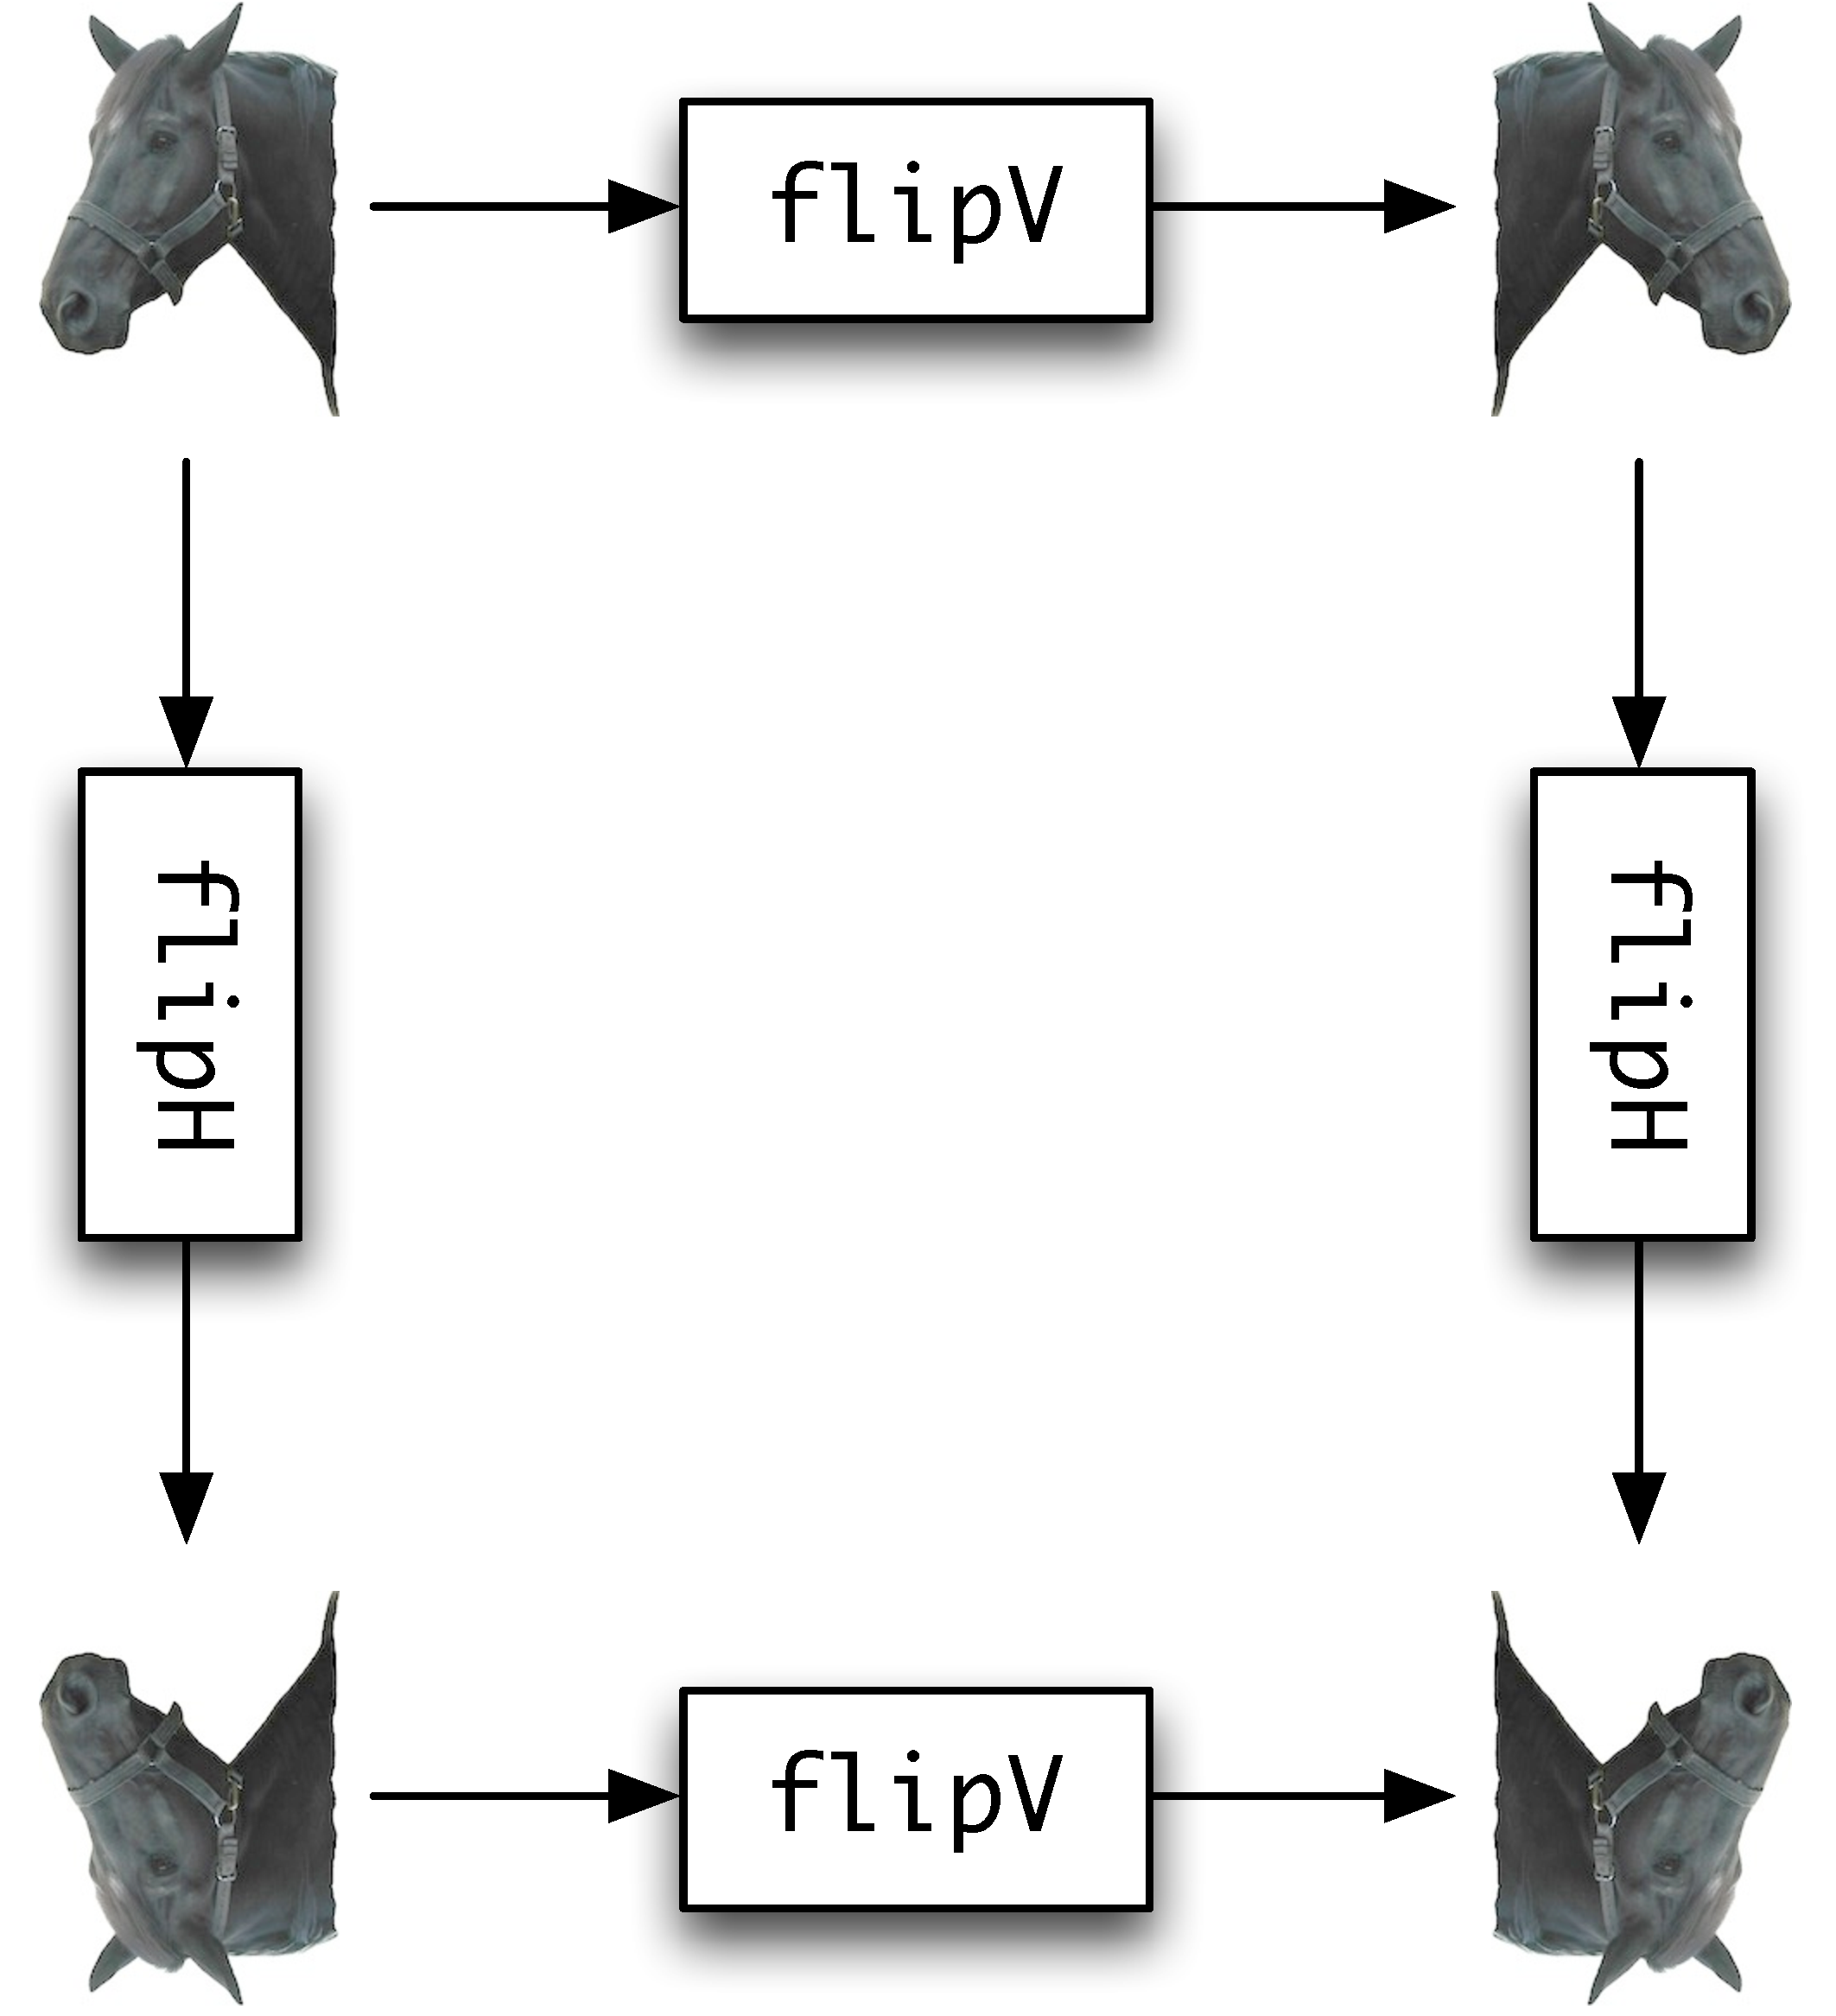
\includegraphics[width=3in]{Pictures/vh-hv.pdf}
\end{center}
\caption{Reflection in vertical and horizontal mirrors}
\label{vh-hv}
\end{figure}
These tests can be defined in Haskell, where the equality operator `\texttt{==}' is used to check whether two values are equal, returning the result \texttt{True} or \texttt{False}. These two values are the two elements of the Boolean type, \texttt{Bool}, which we come back to in the next chapter. Here are the tests:
\begin{alltt}
test_rotate, test_flipV, test_flipH :: Bool
 
test_rotate  =  flipV (flipH horse) == flipH (flipV horse)
test_flipV   =  flipV (flipV horse) == horse
test_flipH   =  flipH (flipV horse) == horse
\end{alltt}\minx{test\_rotate}
The first two tests pass, and give the answer \texttt{True}. The third fails, because we made a mistake in writing \texttt{flipV} when we should have written \texttt{flipH}; if we correct the test, it will pass as well. 


These tests work for a single input, and though \texttt{horse} is as good as any example, we ought to think of making more tests than this. \textbf{Property-based testing} in QuickCheck \cite{quickCheck}\index{QuickCheck} allows us to check whether a property holds for a whole collection of randomly generated inputs. 

What do we mean by a property?\index{property} Informally, it's something like the explanation we gave earlier ``if we flip \emph{a picture} twice in a mirror we expect to get back \emph{the original picture}'' where the ``\emph{picture}'' could be any picture. We can formalise these as Haskell functions:
\begin{alltt}
prop_rotate, prop_flipV, prop_flipH :: Picture -> Bool

prop_rotate pic  =  flipV (flipH pic) == flipH (flipV pic)
prop_flipV pic   =  flipV (flipV pic) == pic
prop_flipH pic   =  flipH (flipV pic) == pic
\end{alltt}\minx{prop\_rotate}

\begin{figure}[t]
\begin{center}
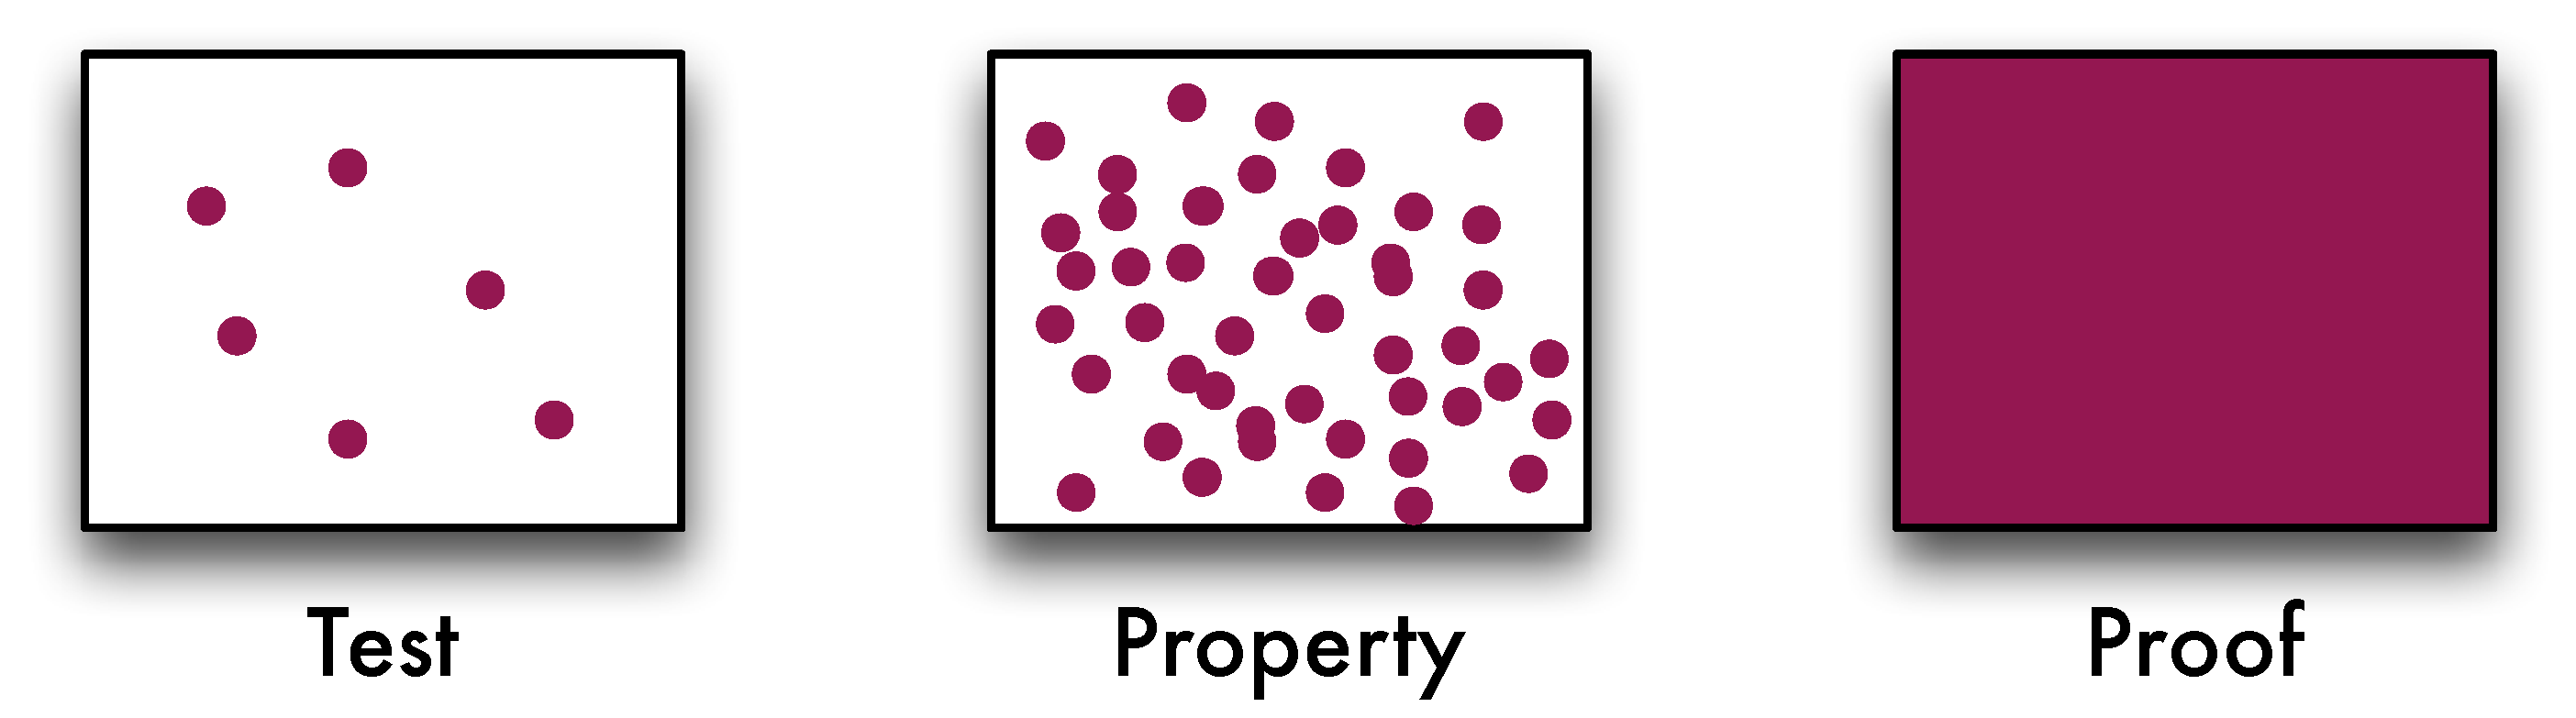
\includegraphics[width=4in]{Pictures/TestPropertyProof.pdf}
\end{center}
\caption{Coverage of testing, property-based testing and proof}
\label{TPP}
\end{figure}

These properties are just like the tests, except that they are applied to an arbitrary \texttt{pic} rather than the \texttt{horse}. If we apply \texttt{quickCheck} to these properties like this
\begin{alltt}
quickCheck prop_rotate
\end{alltt}
and evaluate this in Haskell, we get the result
\begin{alltt}
+++ OK, passed 100 tests.
\end{alltt}
for the first two tests. In the final test we've replicated the error from earlier on, and we get this output
\begin{alltt}
*** Failed! Falsifiable (after 3 tests and 3 shrinks):  
["ab"]
\end{alltt}
This tells us two things: it tells us that the property isn't always true, and it also gives us an example of when it goes wrong. In fact we get the simplest case where it goes wrong, through ``shrinking'':\index{property-based testing!shrinking} this is a picture with one line and two characters!

This testing is automatic: once we have written the properties to test, the data are generated randomly from the type -- \texttt{Picture} in this case. Through the book we'll see more complex examples of using QuickCheck, and find ways that we can control how QuickCheck works. 

\subsection*{Coverage}
\index{testing!coverage}

Property-based testing has replaced one test with a hundred, but we might still be unlucky, and miss the failing cases in the random data. On the other hand, having a proof gives us complete certainty that a function is correct. 

Figure \ref{TPP} illustrates the coverage given by the different mechanisms. Testing will check how the program behaves at a few, well-chosen, points; property-based testing expands this to hundreds of randomly-generated points, which, it is hoped, are representative, but a point where an error occurs \emph{may} be missed\footnote{We'll see an example of this in Chapter \ref{reasoningProgs}}; proof covers \emph{all} cases, no exceptions.

\subsection*{Proof}
\index{proof|(}

A \textbf{proof} is a logical or mathematical argument to show that something
holds {\em in all circumstances}. For example, given any particular
right-angled triangle
\begin{center}
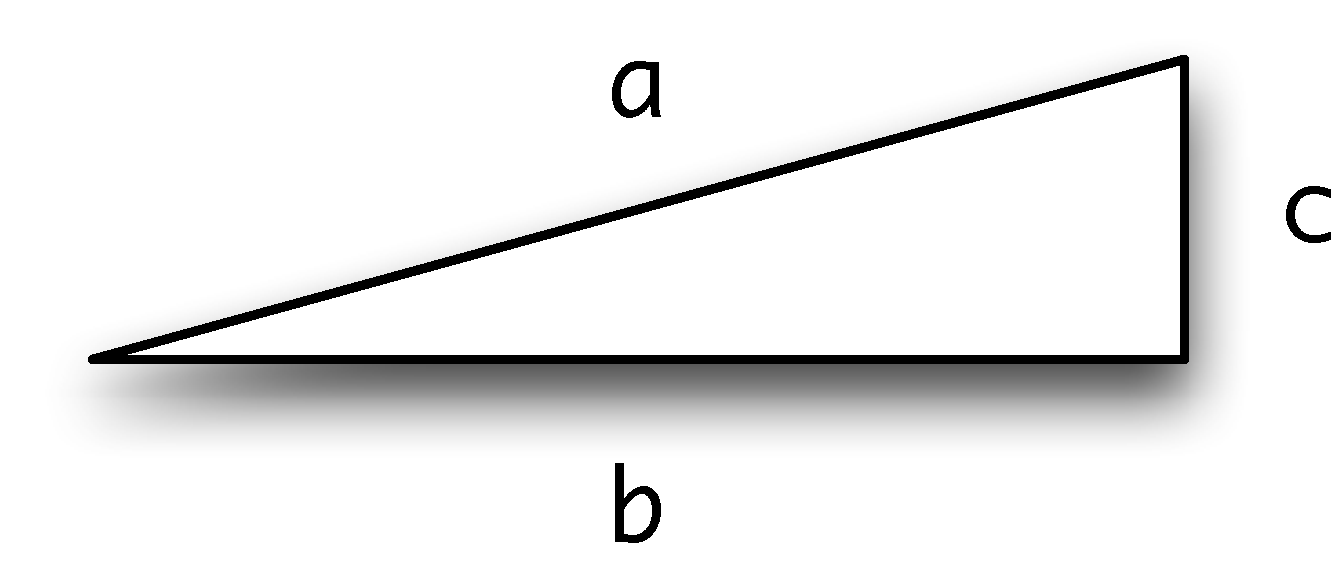
\includegraphics[width=2.0in]{Pictures/pythag.pdf}
\end{center}
we can check whether or not \texttt{a$^{\tt 2}$=b$^{\tt 2}$+c$^{\tt 2}$} holds. 
\index{Pythagoras's theorem} In each case we check,
this formula will hold, but this is not in itself enough to show that the
formula holds for all \texttt{a}, \texttt{b} and \texttt{c}. A proof of Pythagoras's Theorem, on the other hand, is a general
argument which establishes that \texttt{a$^{\tt 2}$=b$^{\tt 2}$+c$^{\tt 2}$} holds whatever
right-angled triangle we choose.

How is proof relevant to functional programming? To answer this we go back to the example of flipping in horizontal and vertical mirrors. As we saw in Figure \ref{vh-hv}, the order of reflection looks as though is not significant, and we can express this as the property:
\begin{alltt}
prop_rotate :: Picture -> Bool
prop_rotate pic  =  flipV (flipH pic) == flipH (flipV pic)
\end{alltt}\minx{prop\_rotate} 
Moreover, we can look at our implementations of
\texttt{flipV} and \texttt{flipH} and give a logical
\textbf{proof}\index{proof} that these functions have the property
\texttt{prop\_rotate} above for \textbf{any} picture \texttt{pic}. The crux of the argument is that the two
functions operate independently:
\begin{itemize}
\item the function \texttt{flipV} affects each line but leaves the lines
in the same order while
\item the function \texttt{flipH} leaves each line unaffected, while
reversing the order of the list of lines.
\end{itemize}
Because the two functions affect different aspects of the list it is
immaterial which is applied first, since the overall effect of applying
the two in either case is to
\begin{itemize}
\item reverse each line and
reverse the order of the list of lines.
\end{itemize}
Proof is possible for most programming languages, but
it is substantially easier for functional languages than for any other
paradigm. Proof of program properties will be a theme in this text, and
we start by exploring proof for list-processing functions in Chapter
\ref{reasoningProgs}.

What benefit is there in having a proof of a property like \texttt{prop\_rotate}?
It give us {\em certainty\/} that our functions have a particular property. 
Contrast this with traditional and property-based testing. In both cases 
the test only gives us the assurance
that the function has the property we seek at the test points, and in principle tells us
nothing about the function in other circumstances. There are
safety-critical situations in which it is highly desirable to be sure
that a program behaves properly, and proof 
has a role here. We
are not, however, advocating that testing is unimportant -- merely that testing
and proof have complementary roles to play in software development. 
 

More specifically, \texttt{prop\_rotate} means that we can
be sure that whatever order we apply the functions \texttt{flipH} and 
\texttt{flipV} they will have the same effect. We could
therefore \textbf{transform}\index{program transformation} a program containing \texttt{...\ (flipH\ (flipV\ ...))\ ...}
into one using the functions in the reverse order,  \texttt{...\ (flipV\ (flipH\ ...))\ ...}, and be certain that the new
program will have exactly the same effect as the old. Ideas like this can be
used to good effect within implementations of languages, and also in
developing
programs themselves, as we shall see in Section \ref{verifGen}.
\index{proof|)}



\begin{summary}
As we said at the start, this chapter has three aims. We wanted to
introduce some of the fundamental ideas of functional programming; to
illustrate them with the example of pictures, and also to give a flavour
of what it is that is distinctive about functional programming.
To sum up the definitions we have seen,
\begin{itemize}
\item a function\index{function} is something which transforms its inputs
to an output;
\item a type\index{type} is a collection of objects of similar sort, such as
 whole numbers (integers)  or pictures;
\item every object has a clearly defined type, and we state this type on
making a definition;
\item functions defined in a program are used in writing expressions to
be evaluated by the implementation; and
\item the values of expressions can be found by
performing calculation by hand, or by using GHCi.
\end{itemize}
In the remainder of the book we'll explore different ways of defining new types
and functions, as well as
following up the topics of polymorphism, functions as arguments and results, data
abstraction and proof which we have touched upon in an informal way
here.
We'll also make sure that we validate our programs using property-based testing in QuickCheck as well as proof. Finally, we'll see how Haskell is used in defining domain-specific languages.
\end{summary}
%\end{document} 



